\ifdefined\included
\else
\documentclass[a4paper,11pt,twoside]{StyleThese}
\usepackage{amsmath,amssymb, amsthm}             % AMS Math
\usepackage[T1]{fontenc}
\usepackage[utf8x]{inputenc}
\usepackage{babel}
\usepackage{datetime}

\usepackage{silence}

\WarningFilter{minitoc(hints)}{W0023}
\WarningFilter{minitoc(hints)}{W0028}
\WarningFilter{minitoc(hints)}{W0030}

\usepackage{lmodern}
\usepackage{tabularx}
%\usepackage{tabular}
\usepackage{multirow}
\usepackage{xspace}

\usepackage{hhline}
\usepackage[left=1.5in,right=1.3in,top=1.1in,bottom=1.1in,includefoot,includehead,headheight=13.6pt]{geometry}
\renewcommand{\baselinestretch}{1.05}

% Table of contents for each chapter

\usepackage[nottoc, notlof, notlot]{tocbibind}
\usepackage{minitoc}
\setcounter{minitocdepth}{2}
\mtcindent=15pt
% Use \minitoc where to put a table of contents

\usepackage{aecompl}

% Glossary / list of abbreviations

\usepackage[intoc]{nomencl}
\iftoggle{ThesisInEnglish}{%
\renewcommand{\nomname}{Glossary}
}{ %
\renewcommand{\nomname}{Liste des Abréviations}
}

\usepackage{etoolbox}
\renewcommand\nomgroup[1]{%
  \item[\bfseries
  \ifstrequal{#1}{A}{Number Sets}{%
  \ifstrequal{#1}{G}{Agents Beliefs and Action Models}{%
  \ifstrequal{#1}{N}{Navigation}{%
  \ifstrequal{#1}{O}{Ontology}{%
  \ifstrequal{#1}{R}{Referring Expression Generation}{%
  \ifstrequal{#1}{Z}{Controllable and Uncontrollable Agents Task Planning}{}}}}}}%
]}

\makenomenclature



% My pdf code

\usepackage{ifpdf}

\ifpdf
  \usepackage[pdftex]{graphicx}
  \DeclareGraphicsExtensions{.jpg}
  \usepackage[pagebackref,hyperindex=true]{hyperref}
  \usepackage{tikz}
  \usetikzlibrary{arrows,shapes,calc}
\else
  \usepackage{graphicx}
  \DeclareGraphicsExtensions{.ps,.eps}
  \usepackage[dvipdfm,pagebackref,hyperindex=true]{hyperref}
\fi

\graphicspath{{.}{images/}}

%% nicer backref links. NOTE: The flag ThesisInEnglish is used to define the
% language in the back references. Read more about it in These.tex

\iftoggle{ThesisInEnglish}{%
\renewcommand*{\backref}[1]{}
\renewcommand*{\backrefalt}[4]{%
\ifcase #1 %
(Not cited.)%
\or
(Cited in page~#2.)%
\else
(Cited in pages~#2.)%
\fi}
\renewcommand*{\backrefsep}{, }
\renewcommand*{\backreftwosep}{ and~}
\renewcommand*{\backreflastsep}{ and~}
}{%
\renewcommand*{\backref}[1]{}
\renewcommand*{\backrefalt}[4]{%
\ifcase #1 %
(Non cité.)%
\or
(Cité en page~#2.)%
\else
(Cité en pages~#2.)%
\fi}
\renewcommand*{\backrefsep}{, }
\renewcommand*{\backreftwosep}{ et~}
\renewcommand*{\backreflastsep}{ et~}
}

% Links in pdf
\usepackage{color}
\definecolor{linkcol}{rgb}{0,0,0.4} 
\definecolor{citecol}{rgb}{0.5,0,0} 
\definecolor{linkcol}{rgb}{0,0,0} 
\definecolor{citecol}{rgb}{0,0,0}
% Change this to change the informations included in the pdf file

\hypersetup
{
bookmarksopen=true,
pdftitle="Planning For Both Robot and Human: Anticipating and Accompanying Human Decisions",
pdfauthor="Guilhem BUISAN", %auteur du document
pdfsubject="Thèse", %sujet du document
%pdftoolbar=false, %barre d'outils non visible
pdfmenubar=true, %barre de menu visible
pdfhighlight=/O, %effet d'un clic sur un lien hypertexte
colorlinks=true, %couleurs sur les liens hypertextes
pdfpagemode=None, %aucun mode de page
pdfpagelayout=SinglePage, %ouverture en simple page
pdffitwindow=true, %pages ouvertes entierement dans toute la fenetre
linkcolor=linkcol, %couleur des liens hypertextes internes
citecolor=citecol, %couleur des liens pour les citations
urlcolor=linkcol %couleur des liens pour les url
}

% definitions.
% -------------------

\setcounter{secnumdepth}{3}
\setcounter{tocdepth}{2}

% Some useful commands and shortcut for maths:  partial derivative and stuff

\newcommand{\pd}[2]{\frac{\partial #1}{\partial #2}}
\def\abs{\operatorname{abs}}
\def\argmax{\operatornamewithlimits{arg\,max}}
\def\argmin{\operatornamewithlimits{arg\,min}}
\def\diag{\operatorname{Diag}}
\newcommand{\eqRef}[1]{(\ref{#1})}

\usepackage{rotating}                    % Sideways of figures & tables
%\usepackage{bibunits}
%\usepackage[sectionbib]{chapterbib}          % Cross-reference package (Natural BiB)
%\usepackage{natbib}                  % Put References at the end of each chapter
                                         % Do not put 'sectionbib' option here.
                                         % Sectionbib option in 'natbib' will do.
\usepackage{fancyhdr}                    % Fancy Header and Footer

% \usepackage{txfonts}                     % Public Times New Roman text & math font
  
%%% Fancy Header %%%%%%%%%%%%%%%%%%%%%%%%%%%%%%%%%%%%%%%%%%%%%%%%%%%%%%%%%%%%%%%%%%
% Fancy Header Style Options

\pagestyle{fancy}                       % Sets fancy header and footer
\fancyfoot{}                            % Delete current footer settings

%\renewcommand{\chaptermark}[1]{         % Lower Case Chapter marker style
%  \markboth{\chaptername\ \thechapter.\ #1}}{}} %

%\renewcommand{\sectionmark}[1]{         % Lower case Section marker style
%  \markright{\thesection.\ #1}}         %

\fancyhead[LE,RO]{\bfseries\thepage}    % Page number (boldface) in left on even
% pages and right on odd pages
\fancyhead[RE]{\bfseries\nouppercase{\leftmark}}      % Chapter in the right on even pages
\fancyhead[LO]{\bfseries\nouppercase{\rightmark}}     % Section in the left on odd pages

\let\headruleORIG\headrule
\renewcommand{\headrule}{\color{black} \headruleORIG}
\renewcommand{\headrulewidth}{1.0pt}
\usepackage{colortbl}
\arrayrulecolor{black}

\fancypagestyle{plain}{
  \fancyhead{}
  \fancyfoot{}
  \renewcommand{\headrulewidth}{0pt}
}

%\usepackage{MyAlgorithm}
%\usepackage[noend]{MyAlgorithmic}
\usepackage{algorithm}
\usepackage[noend]{algpseudocode}
\usepackage{comment}
\usepackage[ED=EDSYS-Robo, Ets=INSA]{tlsflyleaf}
%%% Clear Header %%%%%%%%%%%%%%%%%%%%%%%%%%%%%%%%%%%%%%%%%%%%%%%%%%%%%%%%%%%%%%%%%%
% Clear Header Style on the Last Empty Odd pages
\makeatletter

\def\cleardoublepage{\clearpage\if@twoside \ifodd\c@page\else%
  \hbox{}%
  \thispagestyle{empty}%              % Empty header styles
  \newpage%
  \if@twocolumn\hbox{}\newpage\fi\fi\fi}

\makeatother
 
%%%%%%%%%%%%%%%%%%%%%%%%%%%%%%%%%%%%%%%%%%%%%%%%%%%%%%%%%%%%%%%%%%%%%%%%%%%%%%% 
% Prints your review date and 'Draft Version' (From Josullvn, CS, CMU)
\newcommand{\reviewtimetoday}[2]{\special{!userdict begin
    /bop-hook{gsave 20 710 translate 45 rotate 0.8 setgray
      /Times-Roman findfont 12 scalefont setfont 0 0   moveto (#1) show
      0 -12 moveto (#2) show grestore}def end}}
% You can turn on or off this option.
% \reviewtimetoday{\today}{Draft Version}
%%%%%%%%%%%%%%%%%%%%%%%%%%%%%%%%%%%%%%%%%%%%%%%%%%%%%%%%%%%%%%%%%%%%%%%%%%%%%%% 

\newenvironment{maxime}[1]
{
\vspace*{0cm}
\hfill
\begin{minipage}{0.5\textwidth}%
%\rule[0.5ex]{\textwidth}{0.1mm}\\%
\hrulefill $\:$ {\bf #1}\\
%\vspace*{-0.25cm}
\it 
}%
{%

\hrulefill
\vspace*{0.5cm}%
\end{minipage}
}

\let\minitocORIG\minitoc
\renewcommand{\minitoc}{\minitocORIG \vspace{1.5em}}

\usepackage{multirow}
%\usepackage{slashbox}

\newenvironment{bulletList}%
{ \begin{list}%
	{$\bullet$}%
	{\setlength{\labelwidth}{25pt}%
	 \setlength{\leftmargin}{30pt}%
	 \setlength{\itemsep}{\parsep}}}%
{ \end{list} }

\theoremstyle{definition}
\newtheorem{definition}{Definition}
\renewcommand{\epsilon}{\varepsilon}

% centered page environment

\newenvironment{vcenterpage}
{\newpage\vspace*{\fill}\thispagestyle{empty}\renewcommand{\headrulewidth}{0pt}}
{\vspace*{\fill}}

\usepackage{tablefootnote}

\theoremstyle{plain}
\newtheorem{constraint}{Constraint}[section]

\algnewcommand\algorithmicforeach{\textbf{for each}}
\algnewcommand\algorithmicin{\textbf{in}}
\algdef{S}[FOR]{ForEach}[2]{\algorithmicforeach\ #1\ \algorithmicin\ #2\ \algorithmicdo}

\usepackage{listings}
\lstdefinestyle{customPlan}{
  language=C,
  commentstyle=\itshape\color{green!25!black},
}
\usepackage{pdfpages}

\sloppy
\begin{document}
\setcounter{chapter}{3} %% Numéro du chapitre précédent ;)
\dominitoc
\faketableofcontents
\fi

\chapter{Emulating the Human Decision and Action Processes During Task Planning}
\label{chapter:doublehtn}
\chaptermark{Planning accounting for human decisions}
\minitoc

\section{Introduction}
In the previous chapter, we successfully integrated a verbal communication planner for referring expressions into a multi-agents human-aware task planner. This allows for a communication action containing reference to an object of the environment, to find its feasibility by not relying only on symbolic facts the task planner is manipulating but by precisely determining its content. Moreover, by determining the content of the referring expression, the complexity for the human to understand it can be estimated and is returned as a cost to the task planner. Thus, during the execution, we can avoid many plan failures, repair actions or inefficiency. Although we saw that this approach needs a task planner able to maintain one set of beliefs per agent during the planning process, \acrshort{hatp}, the planner used was only allocating tasks to the human without considering if the human was aware or not of the generated plan.

\acrshort{hatp} is provided with a human model ($\humanmodel$) in several ways. The planning domain contains the actions the humans can perform and their beliefs are updated all along the planning process. Moreover, human preferences can be set on the plan through the \textit{social cost}, adding extra-cost to the plan if some criteria are met such as bad chaining of actions (\textit{e.g.}~the robot mopping the floor just before making a sandwich). However, \acrshort{hatp} assumes that a shared goal has been established between the robot and the human. This shared goal is supposed to have been acquired previously in the interaction, for example via a human request. Besides, as stated before, it generates a plan which is unknown if it needs to be communicated to the human or if it can be easily \textit{guessed} (\textit{i.e.}~which is predictable) by the human. Finally, the plan is ``fixed'' and does not account for whether the human chooses to perform a different path of actions or not. Any deviation of the human from their generated stream of action either needs the supervision to perform repair actions or to request for a replanning. This approach has been shown to be suitable and pertinent in some applications (\textit{e.g.}~when communication can easily be done at any point of the plan).

\smallskip

In this chapter, we present a novel task planning approach dedicated to \acrshort{hri} which, by planning for both the human and the robot, tries to satisfy multiple objectives:

\begin{enumerate}
\item \textbf{Plan without assuming a prior shared goal}. In \acrshort{hri} scenarios, the robot and the human are not always sharing a goal. The robot can for example plan to perform a task around humans that are not involved at first, or it may be requested by a human to do a task without wanting to take a part in it. By doing so, our planner can balance between integrating the sharing of a goal with a human (assumed to be collaborative) in the plan and making the robot do the task alone, or integrate the eventuality to ask for punctual human help.

\item \textbf{Model the human decision processes}. When taking part in a task, a human (assumed willing to collaborate with the robot) will also plan to reach their (potentially shared) goal. Our planner must be able to account for this to provide plans that are expected and explainable by the human partner.

\item \textbf{Help the human decision, but not compel it}. Unlike \acrshort{hatp}, our planner should account for the human flexibility in their decision. While by modeling the human decision processes it is possible to narrow down the possible human actions, the generated plans must be able to help the supervision to avoid to replan or to repair during the execution by considering several human actions.

\item \textbf{Model the potential human reactions}. It is possible to predict that the human may react to some situations, interrupting or helping their current task. We identify two causes of these reactions. First, they can ensue from some specific world states, that have been perceived and interpreted by the human. Then, they can also originate from explicit communications issued by the robot. These communications can either be a belief alignment, updating the human knowledge and impacting their decisions; a request to perform a specific action or a request to help the robot along with a shared goal, needing the human to plan for it.

\item \textbf{Act and decide on the different agents' beliefs}. It is important to be able to represent actions as having different effects on the beliefs of the robot or the human. Indeed, some robot actions are partially or not observable by the human, when performing them, the human has no way of knowing the complete new world state. Besides, these effects and their observability often depend on the current world state, which representation must be supported in the planner. Then, decisions made while planning may require to reason on both the robot and the human beliefs. This is especially the case with communication actions aiming at aligning knowledge or ask questions for example. Finally, some actions of pure decision have no direct effect on the world, but only on the internal beliefs of the agents. For example, observation actions will only update the beliefs of the agent doing it.

\item \textbf{Decide not only on the world state but also on the decision processes of the agents}. Some decisions made during the planning process require access not only to the beliefs of the agents representing the world state, but also to the estimation of their planning processes. For example, the decomposition of a task by the robot may be impossible if some other task is already performed in its partial plan. Other decisions may also need the estimation of the human current planning process. For example, if it has been estimated earlier in the plan that the human will perform a certain decomposition of a task, the planner would assign a complementary task to the robot.

\item \textbf{Adapt to the human experience, trust and preferences}. We also want the planning process to be adjusted depending on the actual human it is planning with. It must perform its plan search differently whether the human has the habit to perform this particular task with the robot or not. Moreover, the human model can be adjusted to the trust the human has in the robot and to their preferences. 
\end{enumerate}

First, we describe our approach and introduce the notations used in this chapter before detailing the planning process. Then, we present the implementation of this approach into a prototype planner in Python that we named \acrfull{hatpehda}. Finally, we demonstrate the planner capabilities in two illustrative situations.

\section{Description}
We separate the agents who may take part in a given task into two categories: the controllable agent (\textit{i.e.}~the robot) for which the planner needs to select the best course of actions to generate a plan; and the uncontrollable agent (\textit{i.e.}~the human) on whom the planner has no direct control but, still, has a representation of their decision, action and reaction models.

The two agent types are fundamentally different: 
\begin{enumerate}
\item the robot is controllable since the process is run by the robot,
\item the human agent is not controllable since the process can only ``speculate'' on their decisions and actions, but can model that the robot actions can still influence them and that some of them are observable by the robot,
\item the two agents are not equivalent, the robot agent role is to help, assist and facilitate human and to synthesize pertinent, legible and acceptable behavior.
\end{enumerate}
We want to devise a planner allowing the controllable agent to plan for its actions while anticipating the decisions, actions and reactions of the uncontrollable agent. Moreover, we want the planner to be able to generate plans where the robot actions elicit situations calling for human decision, action and reaction, thus creating and anticipating collaboration and interaction.

\smallskip

This problem may be seen as a classical non deterministic planning problem, but enriched with the ability of the robot to model the actions, beliefs and decision process of the human. Thus, we have to consider distinct action models, beliefs and execution streams for each of the agents involved. Doing so with classical STRIPS-style planning approaches would potentially lead to an intractable search space. Moreover, \acrshort{htn} approaches have already been shown to be suitable for \acrshort{hri} as they allow to communicate about the plan more easily~\cite{lallement2014hatp}. Therefore, we chose to use \acrshort{htn} planning for both the controllable and uncontrollable agents. \acrshort{htn} planning aims at decomposing abstract tasks into atomic primitive tasks by choosing from a list of available context-dependent refinements for each abstract task, ensuring that preconditions and effects of refined primitives tasks are satisfied throughout the created plan. Similarly to HATP~\cite{sebastiani2017dealing}, our planner elaborates a plan with several streams of actions each assigned to an agent involved in the task. But while in \acrshort{hatp}, all the streams are built starting from on initial root node corresponding to a shared goal between all agents, our planner starts from multiple initial root nodes corresponding to the decision process of the different agents.

The main structure manipulated by our planner is the \textbf{agent}, more precisely two will be represented, the \textit{human} and the \textit{robot}. Each agent has their own \textbf{beliefs}, \textbf{action model}, \textbf{agenda}, \textbf{plan} and \textbf{triggers}. The planner has to use their action models and beliefs to decompose the tasks in their agenda into primitive tasks (actions) that are inserted in their plan. By doing so, it also has to update the beliefs of each agent and to model their reaction by executing the triggers.

\paragraph{\bf Agents:}
First, we define an agent state as a tuple $\agentstate_{\agent} = \langle  \agenda_{\agent}, \plan_{\agent}, \worldstate_{\agent} \rangle$, with $\agenda_{\agent}$ the agenda, $\plan_{\agent}$ the partial plan and $\worldstate_{\agent}$ of the agent $\agent$ (more details are presented in what follows). Then, we define an agent as being $\agent = \langle \text{name}_{\agent}, \agentstate_{\agent}, \actionmodel_{\agent}, \triggerset_{\agent} \rangle$, with $\text{name}_{\agent}$ the agent name, $\agentstate_{\agent}$ the agent state, $\actionmodel_{\agent}$ the action model and $\triggerset_{\agent}$ the triggers of the agent $\agent$ (detailed in what follows). Then we define two agents: the controllable one --- the \textit{robot} ---; and the uncontrollable one --- the \textit{human} ---. We have $\agentstate = \langle \agentstate_{robot}, \agentstate_{human} \rangle$ representing an agent\textbf{s} state, being the state of all the agents at a certain plan step. Let $\agentsstatesset$ be the set of all the possible agents states.

\paragraph{\bf Beliefs:}
Let $\statespace$ be the set of all possible world states, we call beliefs of an agent $\agent$ the state $\worldstate_{\agent} \in \statespace$ in which this agent thinks the world is in. It is important to note that the state of the controllable agent (robot) is assumed to be the real world state estimation for the planner, as we consider the planner as being part of the controllable agent.

\paragraph{\bf Action models:}
We represent the action model of an agent $\agent$ as $\actionmodel_{\agent} = \langle \operators_{\agent}, \abstracttasks_{\agent}, \methods_{\agent} \rangle$ where $\operators_{\agent}$ are the primitive tasks (\textit{i.e.}~operators, actions) that the agent $\agent$ can perform, $\abstracttasks_{\agent}$ the set of abstract tasks and $\methods_{\agent}$ are the methods (\textit{i.e.}~decompositions) describing how an agent $\agent$ can perform an abstract task through a refinement process. It is important to note that while this representation makes a clear distinction between the robot and the human tasks, it does not prevent representing joint abstract tasks or tasks that can be either done by one or the other agent. Indeed, as we show later, complementary abstract tasks can be represented and some tasks can have the same operational model even if they are not in the same agent action model. 

More precisely, the primitive tasks (operators) are defined as functions: $\operators \ni o: \agentsstatesset \rightarrow \agentsstatesset \cup \bot$ which produce new agents state, being the effect of the application of the primitive task, or \textit{false} if the task is not applicable. We represent operators as being instantaneous (or all having the same duration) in their realization. In the future, to represent more accurately intricate coordination, we want to include the expected duration of an operator.

Then, methods are defined as tuple, containing an abstract task and a decomposition function: $\methods \ni m = \langle \alpha, \delta \rangle$ with $\alpha \in \abstracttasks$ and $\delta: \agentsstatesset \rightarrow (\operators \cup \abstracttasks)^n \cup () \cup \bot$ with $n \in \intset^*$, which, depending on agents states, decompose the abstract task returning a sequence of tasks (primitive or abstract), an empty sequence if the abstract task does not need to be decomposed, or \textit{false} if the task cannot be decomposed in the current state. Multiple methods can address the same abstract task, the goal of the HTN planner is then to choose the right one to create a plan.

\paragraph{\bf Agents agendas and plans:}
An agenda $\agenda_{\agent}$ and a plan $\plan_{\agent}$ (this agent only stream of actions) are defined for each agent $\agent$. The agenda $\agenda_{\agent}$ is a sequence of tasks (abstract or primitive) having to be performed by the agent. The plan $\plan_{\agent}$ is a sequence of primitive tasks, built from the agenda, which the agent has to perform. The links of actions order between the two streams of actions (plans) are kept in each plan, allowing for coordination.

\paragraph{\bf Agent triggers:}
Finally, we define for each agent $\agent$ a set of so-called \textit{trigger functions} $\triggerset_{\agent}$. These trigger functions aim at representing reactions of agents to certain situations (subsets of world states). They are useful to model event-driven behavior, as in PRS~\cite{ingrand1996prs}, when a specific world state \textit{triggers} a reaction from an agent. Besides, these triggers can be used to represent social norms as defined in \cite{carlucci2015explicit}, where the user can specify literals which, if true in the world state during the planning process, add some specific robot actions to the plan.

Trigger functions are defined as: $\triggerset \ni t: \agentsstatesset \rightarrow (\operators \cup \abstracttasks)^n \cup ()$ with $n \in \intset^*$, returning a sequence of tasks to be inserted in an agent agenda as a reaction to specific agent states. For now, the tasks returned by a trigger function are added on top of the agenda, thus preempting any task that may have started to be decomposed. A considered solution is to support the flagging of some abstract tasks in the domain as being \textit{atomic}. We can then prevent the tasks returned by a trigger to be inserted between any tasks resulting from the decomposition of an atomic task.

\section{The Proposed Planning Process}
The cooperative agents planning problem consists of two agents $\agents_{start}$ with their respective agenda filled with tasks to achieve and their beliefs about the current world. For the controllable agent (\textit{i.e.}~the robot), the beliefs correspond to the planner ground truth, for the uncontrollable agent, their beliefs need to be estimated, through, for example, situation assessment component~\cite{milliez2014framework, lemaignan2018underworlds}. Both beliefs are then updated separately during the planning process, allowing to detect and correct belief divergences for example. 

The result is a robot conditional plan $\policy$ being a tree of alternating robot and human primitive tasks. Any path from the root to the leaves is a feasible sequence of primitive tasks (\textit{i.e.}~each primitive task application leads to a state where the following one is applicable) leading to a state where the robot agenda is empty\footnote{We also intend to make the planner stops at a certain depth. Thus, it could be used during the execution to plan a few steps ahead but not until the task is over.}

To solve such a problem we need to augment the search space from world states $\statespace$ only to all the agents states considered by the planner $\agentsstates$, with their agenda, plan and beliefs. The exploration starts with $\agentsstates^{start}$ and consecutively applies operators associated to the robot and to the human, leading to new agents states $\agentsstates^{i}$ until the controllable agent has an empty agenda: $\agenda_{robot} = ()$.

The search, which will be detailed after, is done in two parts:
\begin{enumerate}
\item First, the robot and human HTNs are explored to find all the feasible plans (and in future works, also all the failing plans). This first exploration results in a tree of alternating robot and human primitive tasks but where robot ones are not selected yet (in the tree, several robot actions can be issued after a human one). Moreover, this tree has an additional dimension corresponding to the task hierarchy originating from the \acrshortpl{htn} decompositions.

\item  Then, a conditional plan is selected from this tree. The conditional plan is also a tree of alternating human and robot primitive tasks, but the robot tasks have been selected (according to cost functions detailed later in this chapter) so only one robot primitive task can follow a human one (\textit{i.e.}~the human primitive tasks now have only one child).
\end{enumerate}

Again, the generated conditional plan keeps the task hierarchy of the \acrshortpl{htn} decomposition, allowing the supervision component to more easily communicate about it, to be reasoned on, or to be stored with a semantic meaning for it to be reused later in other components. Selecting robot actions while still accounting for the possible human ones allows for simpler plan post-processing at the execution. For example, Levine and Williams propose to let the robot action choices and causality analysis to the execution~\cite{levine2014concurrent}. While with this approach repairing plan is easier, the execution component may not have all the information to make decisions.

\subsection{Action Models Restriction}


Some constraints on the operator, method and trigger functions must be respected. Indeed, depending on whether the agent is controllable or not, their planning process will not take decisions based on the same information, and their action will not impact the world state in the same manner. We thus impose restrictions on what a function can read and write (writing means here having effects on agents states and is only in the case of primitive task functions) in the agents state. Then, the function constraints also depend on which agent is performing the action or making the decision (in method and trigger functions). The rules for read and write accesses are given in Table~\ref{table:function_restrictions}. 

\begin{table}[htb]
\centering
\begin{tabular}{|c||c|c|} 
 \hline
 Agent type & Readable & Writable \\
 \hline
 Controllable (robot) & \begin{tabular}[c]{@{}l@{}}$\worldstate_{robot}, \worldstate_{human},$ \\ $\plan_{robot}, \plan_{human}$ (a)\end{tabular} & \begin{tabular}[c]{@{}l@{}}$\worldstate_{human}, \worldstate_{robot},$(b)\\ $\agenda_{human}, \agenda_{robot}$ (c)\end{tabular}\\
 \hline
 Uncontrollable (human) & $\worldstate_{self}, \plan_{self}$ (d) & $\worldstate_{self}, \worldstate_{other}, \agenda_{self}$ (e)\\
 \hline
\end{tabular}
\caption{Readable and writable elements (belief states, agenda, plan) of the agents state by method, primitive task and trigger functions.}
\label{table:function_restrictions}
\end{table}

\paragraph{Table~\ref{table:function_restrictions}(a):} During robot planning, the decision and the action can depend on the beliefs of the robot and on the planned estimated beliefs of the human. Moreover, the current partial plan of the robot and the anticipated plan of human one can also be used to make decisions.

\paragraph{Table~\ref{table:function_restrictions}(b):} The effects of robot actions obviously impact its own belief state (considered as the real world state by the planner), but also the beliefs of the human, for example, through their observation process and first order logic reasoning. More elaborate schemes to compute the effects can also be devised such as those described in~\cite{gharbi2015combining}.

\paragraph{Table~\ref{table:function_restrictions}(c):} Besides, a robot action can add a new task to the agenda of the human. This is to account for communication actions requesting the human to do something.

\paragraph{Table~\ref{table:function_restrictions}(d):} The human decisions and actions can only be done according to her own beliefs and partial plan. Indeed, we cannot add the robot ones as it is, or we would consider that the human estimation of the robot knowledge and past actions is always perfect. This would require a third type of agent, being the robot model as estimated by our estimation of the human. For now, we chose not to represent the estimation of the robot partial plan in the human beliefs. Indeed, it would require to reason on the observability of the robot actions to represent them in the human beliefs. However, the human beliefs can be updated through robot actions.

\paragraph{Table~\ref{table:function_restrictions}(e):} The effects of the human actions obviously impact their beliefs and the robot (planner) ones. Moreover, the human agenda could also be updated through, for example, a positive answer to a task request.


\subsection{Exploration Algorithm}
Our planner operates in a turn-taking scheme, based on the update of the agents' beliefs states, the \acrshortpl{htn} of the robot and the human are explored successively.

\subsubsection{Controllable Agent HTN Exploration}
The robot \acrshort{htn} exploration is a pretty standard depth-first algorithm presented in Algorithm~\ref{alg:seek_plans}. The first task $\lambda$ from its agenda $\agenda_{robot}$ its popped, then if it is an abstract task $\lambda \in \abstracttasks$, all the applicable methods are applied, and their results are prepended to the agenda, thus giving new agents states (with the same beliefs as the previous ones but with the robot agenda updated) and branching our search space. We iterate with the new task popped from the new robot agenda. Eventually, the popped task will be a primitive one $\lambda \in \operators$, its function will then be applied to the currently explored agent states. If it returns \textit{false}($\bot$), the action is not applicable, and the exploration backtracks to another decomposition of an abstract task. However, if the action is applicable (returns a new agents state), the triggers are run for each agent, updating their agenda if necessary. Then, we question the human \acrshort{htn} to get their possible next actions from this new agents state, and, for each possible new agents state, we apply the triggers of each agent then we continue the robot \acrshort{htn} exploration. This exploration continues until the robot agenda is empty, or all the branches return \textit{false}.

\begin{algorithm}[htb!]
\begin{algorithmic}[1]
\Function {SeekPlans}{$robot$, $human$}
\State $solutions \leftarrow$ an empty list of plans
\State $result \leftarrow \textsc{ExploreTree}(robot, human, solutions)$
\If {$result =$ failure} \Return failure \EndIf
\State \Return $solutions$
\EndFunction
\Statex
\Function {ExploreTree}{$r$, $h$, $solutions$}
\If {$\textsc{isEmpty}(\agenda_r)$}
	\State add the plan $\plan_r \cup \plan_h$ in $solutions$
	\State \Return success
\EndIf
\State $\lambda \leftarrow \textsc{Pop}(\agenda_r)$
\If{$\lambda \in \abstracttasks_r$}
	\State $isOneDecompositionValid \leftarrow$ false
	\ForEach{$\langle \alpha, \delta \rangle$}{$\methods_r$ s.t. $\alpha = \lambda$}
		\State $decomposition \leftarrow \delta(\worldstate_r, \plan_r, \agenda_r, \worldstate_h, \plan_h, \agenda_h)$
		\If {$decomposition \neq \bot$}
			\State $r', h' \leftarrow \textsc{Copy}(r, h)$ \Comment{The exploration is branching on the robot decompositions, so we deep copy the agents to avoid interactions between branches}
			\State $\agenda_{r'} \leftarrow decomposition.\agenda_{r'}$
			\State $result \leftarrow \textsc{ExploreTree}(r', h', solutions)$
			\If {$result =$ success}
				$isOneDecompositionValid \leftarrow$ true
			\EndIf
		\EndIf
	\EndFor
	\If {$isOneDecompositionValid$} \Return success \EndIf
\EndIf
\If{$\lambda \in \operators_r$}
	\State $result \leftarrow \lambda(\worldstate_r, \plan_r, \agenda_r, \worldstate_h, \plan_h, \agenda_h)$
	\If {$result = \bot$}
		\Return failure
	\EndIf
	\State $r', h' \leftarrow \textsc{Copy}(r, h)$ \Comment{The exploration is branching on the human operators, so we deep copy the agents to avoid interactions between branches}
	\State $\worldstate_{r'}, \agenda_{r'}, \worldstate_{h'}, \agenda_{h'} \leftarrow \textsc{Apply}(result)$
	\State $\plan_{r'} \leftarrow \plan_{r'}.\lambda$
	\State $\agenda_{r'}, \agenda_{h'} \leftarrow \textsc{ApplyTriggers}(\worldstate_{r'}, \plan_{r'}, \agenda_{r'}, \worldstate_{h'}, \plan_{h'}, \agenda_{h'})$
	\State $humanApplicableOperators \leftarrow \textsc{GetHApplicableOperators}(h')$
	\State $isOneOperatorValid \leftarrow$ false
	\ForEach{$o$}{$humanApplicableOperators$}
		\State $r'', h'' \leftarrow \textsc{Copy}(r', h')$
		\State $\worldstate_{r''}, \worldstate_{h''}, \agenda_{h''} \leftarrow \textsc{Apply}(o)$
		\State $\agenda_{r''}, \agenda_{h''} \leftarrow \textsc{ApplyTriggers}(\worldstate_{r''}, \plan_{r''}, \agenda_{r''}, \worldstate_{h''}, \plan_{h''}, \agenda_{h''})$
		\State $result \leftarrow \textsc{ExploreTree}(r'', h'', solutions)$
		\If {$result =$ success} $isOneOperatorValid \leftarrow$ true \EndIf
	\EndFor
	\If {$isOneOperatorValid$} \Return success \EndIf
\EndIf
\EndFunction
\end{algorithmic}
 \caption{Double HTN main exploration algorithm.}
  \label{alg:seek_plans}
\end{algorithm}

\subsubsection{Uncontrollable Agent HTN Exploration}
The human \acrshort{htn} exploration differs from classical HTN planner as the goal is not to produce a complete plan, but rather to list all the actions the human is likely to perform in a given agents state. As presented in Algorithm~\ref{alg:gethactions}, we recursively decompose the first task of the human agenda $\agenda_{human}$ with every applicable method, until we reach an applicable operator. All the operators from all the applicable decompositions are returned to the robot \acrshort{htn} exploration and applied.

\begin{algorithm}[htb!]
\begin{algorithmic}[1]
\Function {GetHApplicableOperators}{$h$}
\State $solution \leftarrow ExploreApplicableOps(h)$
\If {$solution = ()$}
	\Return $(WAIT)$
\EndIf
\EndFunction
\Statex
\Function{ExploreApplicableOps}{$h$}
\If{$\textsc{isEmpty}(d_h)$}
	\Return $(IDLE)$
\EndIf
\State $\lambda \leftarrow \textsc{Pop}(\agenda_h)$
\If {$\lambda \in \abstracttasks_h$}
	\State $applicableOps \leftarrow$ an empty set of operators
	\ForEach{$\langle \alpha, \delta \rangle$}{$\methods_h$ s.t. $\alpha = \lambda$}
		\State $decomposition \leftarrow \delta(\worldstate_h, \plan_h)$
		\If {$decomposition \neq \bot$}
			\State $h' \leftarrow \textsc{Copy}(h)$
			\State $\agenda_{h'} \leftarrow decomposition.\agenda_{h'}$
			\State $applicableOps \leftarrow applicableOps \cup ExploreApplicableOps(h')$
		\EndIf
	\EndFor
	\State \Return $applicableOps$
\EndIf

\If{$\lambda \in \operators_h$}
	\If{$\lambda(\worldstate_h, \plan_h, \agenda_h) \neq \bot$}
		\State \Return $\{\lambda\}$
	\Else
		\State \Return an empty set
	\EndIf
\EndIf
\EndFunction
	
\end{algorithmic}
 \caption{Human HTN exploration algorithm, returning the feasible human actions.}
 \label{alg:gethactions}
\end{algorithm}

\subsubsection{Default Actions} Two special cases are handled during the exploration. If the human agenda is empty whereas the robot one is not, the exploration returns a default action \textit{IDLE} --- which does not modify agents beliefs nor agendas --- for the human. This action represents the non-involvement of the human in a task. Besides, if for the human no applicable action is found a default action \textit{WAIT} --- which does not modify agents nor agendas --- is returned. This action represents the impossibility of the human to act in the current situation, making them wait for the robot to proceed. This default action can also be used in a domain to represent the human decision to wait for the robot to act.

Once the robot agenda is emptied, the agents state is set as a success, the plan is added to the valid plans tree and the search can be continued until no decomposition is left for any task.


\subsection{Conditional Plan Selection}
Once this exhaustive search has been done, the result is a valid plans tree of alternating robot and human feasible actions along with their current beliefs leading to a task completion. For simplicity we will represent the function returning the children of each operator in this tree as $\textsc{NextActions}: \operators \mapsto \mathcal{P}(\operators)$. More precisely, as the agents of the action alternate between the robot and the human we have $\textsc{NextActions} \in \mathcal{P}(\operators_{human})^{\operators_{robot}} \cup \mathcal{P}(\operators_{robot})^{\operators_{human}}$ (a robot action can only have human actions as children and a human action can only have robot actions as children). 

The goal of this second planning step is to select robot actions such as each human action in the plan has only one robot action as a child.
To do so, we define a cost function $cost: \agentsstates \times \operators \mapsto \realset^+$ representing the cost of an action in a specific state. The data structure is now similar to a two players game tree. However, \textit{MinMax} approaches are not suitable here, as we are not in an adversarial setup but more into a collaborative one. Indeed, trying to minimize the maximal possible cost is assuming that the human will always do the actions leading to the worst plan. This defensive behavior could lead to non optimal plans. We assume that given the right indications, the human will do their best to achieve the task with minimal cost. We thus propose to explore this tree differently.

Moreover, like in \acrshort{hatp} we allow to define \textit{social costs} functions. These functions take a complete human and robot sequence of actions ($\plan_r$ and $\plan_h$) and return a cost ($\realset^+$) which is added to the cost of the plan previously determined. By doing so, we can penalize non acceptable sequence of robot actions (\textit{e.g.}~serving a meal just after taking out the trash) or non satisfactory human required contribution (\textit{e.g.}~a plan requiring the human to act after a long series of \textit{IDLE} actions, meaning the human could have disengaged from the task; or requesting the human to perform small tasks multiple times instead of giving the big picture of the real task to perform).

\paragraph{Minimizing the Average Cost}
The approach we propose for plan selection is to minimize the average cost (Algorithm~\ref{alg:minaverage}). It represents the human potentially selecting any course of actions in their stream (while still respecting the action model defined in their \acrshort{htn}).

The algorithm is given the root action of the task network previously generated and returns the cost of the conditional plan selected while having selected the robot actions in the task network. The functions used in Algorithm~\ref{alg:minaverage} are described hereafter:

\begin{itemize}
\item \textbf{\textsc{PathEndingWith}}: This function recursively backtracks from an action to get all its parents. This results in a path in the conditional plan tree, \textit{i.e.}~a plan as a sequence of alternating human and robot actions on which a social cost can be computed.

\item \textbf{\textsc{PerformingAgent}}: This function returns the agent performing the action given as argument (either the robot or the human).

\item \textbf{\textsc{ApplicationState}}: Return the state $\agentsstates$ on which the action given as argument is applied.
\end{itemize}

While this is a first step and additional work is required for conditional plan selection, it has proven to work on several examples shown later in this chapter.

\begin{algorithm}[htb]
\begin{algorithmic}[1]
\Function{SelectRobotActions}{$action$, $actualCost$}
\If{$\textsc{NextActions}(action) = \bot$} \Comment{If it is the last action, we compute the social cost of the plan and return its addition with the per-action cost.}
	\State $actualCost \leftarrow actualCost + \textsc{Cost}(\textsc{ApplicationState}(action), action)$
	\State \Return $actualCost$ + $\textsc{SocialCost}(\textsc{PathEndingWith}(action))$
\EndIf
\If{$\textsc{PerformingAgent}(action) =$ robot} \Comment{If this action is done by the robot, its direct children are performed by the human}
	\State $totalCost \leftarrow 0$
	\State $actionCost \leftarrow \textsc{Cost}(\textsc{ApplicationState}(action), action)$
	\ForEach{$child$}{$\textsc{NextActions}(action)$}
		\State $totalCost \leftarrow \textsc{SelectRobotActions}(child,$\\
		\hfill$actualCost + actionCost)$
	\EndFor
	\State \Return $totalCost / \textsc{Card}(\textsc{NextActions}(action))$
\Else{} \Comment{This action is done by the human, its direct children are done by the robot and need to be selected}
	\State $minCost \leftarrow +\infty$
	\State $chosenChild \leftarrow$ null
	\State $actionCost \leftarrow \textsc{Cost}(\textsc{ApplicationState}(action), action)$
	\ForEach{$child$}{$\textsc{NextActions}(action)$}
		\State $childCost \leftarrow \textsc{SelectRobotActions}(child,$\\
		 \hfill$actualCost + actionCost)$
		\If{$actionCost < minCost$}
			\State $minCost \leftarrow childCost$
			\State $chosenChild \leftarrow child$
		\EndIf
	\EndFor
	\State Set the result of $\textsc{NextActions}(action)$ to $chosenChild$
	
	\State \Return $minCost$	
\EndIf
\EndFunction
	
\end{algorithmic}
 \caption{Conditional plan selection algorithm. Explores a search space (a bipartite tree of alternating robot and human actions) to choose the robot actions minimizing the average of the total plan cost over all the possible human actions.}
 \label{alg:minaverage}
\end{algorithm}

This method for selecting a conditional plan is quite simple but is enough to show the principles and how the approach can be useful for planning in \acrshort{hri}. We propose other methods of plan selection, accounting even more on the human modeling, which have yet to be refined in Section~\ref{subsec:chap4selectingplan}.

\section{Implementation}
The previous section presented the general ideas and concepts behind this new planning paradigm. This short section shows some interesting details about the actual implementation of a prototype of the planner, along with some explanations preparing the following examples presentation. We named this prototype planner \acrfull{hatpehda}. In the next chapter, we will also show how it has been integrated with other components to extend its capabilities and be used in a real robotic architecture.

\subsection{A Python Planner}
We chose to implement \acrshort{hatpehda} in Python\footnote{This prototype is available, as work in progress, at \url{https://github.com/guilhembn/HATPEHDA} along with the example presented in this chapter, and the interfaces with the other components presented in the following chapter.}. It is originally based upon the \acrfull{pyhop} from Nau but has been largely modified, and only remain the general data structures. As in \acrshort{pyhop}, it allows to represent world states as Python objects having dictionary as attributes. For example \verb|s.isReachableBy["cube_23"] = ["human_3", "pr2_robot"]| specifies that the \textit{cube\_23} is reachable by both the \textit{human\_3} and the \textit{pr2\_robot}. 
%A more detailed state representation with a beliefs divergence is available in Listing~\ref{list:pystatedef}.
Moreover, like in \acrshort{pyhop} the planning domains (\acrshortpl{htn} for both the robot and the human) are written using plain Python functions. While using a separate domain-specific language (DSL) for writing planning domains enables some optimizations and advanced search algorithms, it tremendously reduces the expressiveness and makes representing real worlds scenarios more complex. Besides, Python being an interpreted language, iterating over these domains is quicker as, unlike \acrshort{hatp}, they do not require any compiling before being planned upon.
The decomposition functions take the world states (beliefs), partial plans of the agents (depending on the type of the agent~Table~\ref{table:function_restrictions}) and any other optional parameters (\textit{e.g.}~goals, entities) as arguments, and return a list of tasks with optional parameters to be put in the agent's agenda. Likewise, the actions receive as arguments the world states (beliefs), the partial plans and the agendas of the agents (also depending on the type of the agent~Table~\ref{table:function_restrictions}) and return new world states and agendas.

The search algorithms have also been implemented in Python. A lot of optimization can be done, and it is planned to entirely rewrite the software in C++. The current prototype, while not being efficient compared to other approaches, still allows to find plans in a reasonable time for realistic human robot scenarios.

\definecolor{greenstring}{RGB}{6, 125, 23}
\definecolor{bluekeyword}{RGB}{0, 51, 179}
\definecolor{greycomment}{RGB}{140, 140, 140}
\lstset{frame=tb,
  language=Python,
  breaklines=true,
  showstringspaces=false,
  columns=flexible,
  numbers=none,
  commentstyle=\color{greenstring},
  stringstyle=\color{greenstring},
  basicstyle=\small\tt,
  keywordstyle=\color{bluekeyword},
  commentstyle=\color{greycomment},
}

\begin{comment}
\begin{lstlisting}[language=Python, caption={Initial states definition for the robot and for the human. A beliefs divergence is represented as being the estimation of the human not knowing that the robot is holding the \textit{mug\_0}.}, label={list:pystatedef}]
[...]
state_r = State('robot_init')
state_r.individuals = {'Mug': ['mug_0', 'mug_1'], 'Agent': ['human', 'robot']}
state_r.isHeldBy = {'mug_0': ['robot'], 'mug_1':[]}
state_r.isHolding = {'human': [], 'robot': ['mug_0']}
state_r.isOwnedBy = {}
state_r.isNotOwnedBy = {}
state_r.isReachableBy = {'mug_0': ['human', 'robot'], 'mug_1': ['human', 'robot']}

state_h = State('human_init')
state_h.individuals = {'Mug': ['mug_0', 'mug_1'], 'Agent': ['human', 'robot']}
state_h.isHeldBy = {'mug_0': [], 'mug_1':[]}
state_h.isHolding = {'human': [], 'robot': []}
state_h.isOwnedBy = {}
state_h.isNotOwnedBy = {}
state_h.isReachableBy = {'mug_0': ['human', 'robot'], 'mug_1': ['human', 'robot']}
[...]
\end{lstlisting}

\begin{lstlisting}[language=Python, caption={}, label={}]
[...]
def pick_mug(self_agent, other_agent, mug):
	# This action is intended to be a robot action
	# The first two parameters are common to every operator function
	# self_agent: contains the robot beliefs (state), id (name), plan and agenda as attributes
	# other_agent: contains the human beliefs (state), id (name), plan and agenda as attributes
	# Then, additional arguments of any type can be provided
	# mug: the mug id to pick
    if self_agent.name in self_agent.state.isReachableBy[mug] and self_agent.state.isHolding[self_agent.name] == []:
		# Update the robot beliefs
		self_agent.state.isReachableBy[mug] = []
        self_agent.state.isHolding[self_agent.name] = [mug]
        self_agent.state.isHeldBy[mug] = [self_agent.name]   
        
        # Update the other agent beliefs only if they are in the same room
    	robot_room = self_agent.state.isInRoom[self_agent.name][0]  # The room in which the robot is
        if self_agent.state.isInRoom[other_agent.name][0] == robot_room
            other_agent.state.isReachableBy[mug] = []
            other_agent.state.isHolding[self_agent.name] = [mug]
            other_agent.state.isHeldBy[mug] = [self_agent.name]
        return self_agent, other_agent
    return False  # If the preconditions are not met, the function returns False
[...]
\end{lstlisting}
\end{comment}

\subsection{Drawing the Plans}
Thinking about the robot programmer is almost as important as considering the human partner the robot will interact with. Thus, in order to debug the designed \acrshortpl{htn}, we provide a way of visualizing the valid plans tree and the generated conditional plan. 

An example of visualization of valid plans tree (before selecting a conditional plan) is presented in Figure~\ref{fig:chap4mugsss}. The ellipses correspond to primitive tasks while rectangles represent abstract ones. The octagons represent the default actions (\textit{IDLE} and \textit{WAIT}). The blue shapes are robot tasks and the yellow ones are the human ones. Finally, red arrows indicate the sequence of actions in the plans and gray ones represent hierarchical links, \textit{i.e.}~the links between the tasks as defined in the \acrshortpl{htn}, along with the decomposition numbers next to them.

It is interesting to note that in Figure~\ref{fig:chap4mugsss} some human actions are followed by two potential robot actions (yellow shapes of which originate red arrows leading to several blues shapes). Indeed, these actions are feasible by the robot, but no plan has been selected yet. Whereas in Figure~\ref{fig:chap4mugtrialerror}, representing a conditional plan selected from the previous figure, the robot actions are set, and the non determinism is only on the human actions.

\section{Examples}
In this section, we will present some case studies in which are presented small task examples. Each example will present some features of the planner and comparisons between multiple plans depending on some initial conditions (beliefs or action costs). Besides, they will give insights into the rationale used when creating the domains for both the robot and the human. The Python domains for both examples are available in Annex~\ref{annex:codedomains}.



The two following cases are set in the same context presented in Figure~\ref{fig:chap4coffeescene}. We envision a super-scenario in a company office where a robot assistant is verbally requested by a human worker to bring her a coffee. The robot must take her mug, go to the coffee machine, manage to fill the mug with coffee and bring back the filled mug to the worker.
We instantiate this scenario into two precise subtasks highlighting multiple features of \acrshort{hatpehda}.

\begin{figure}[hbtp]
\centering
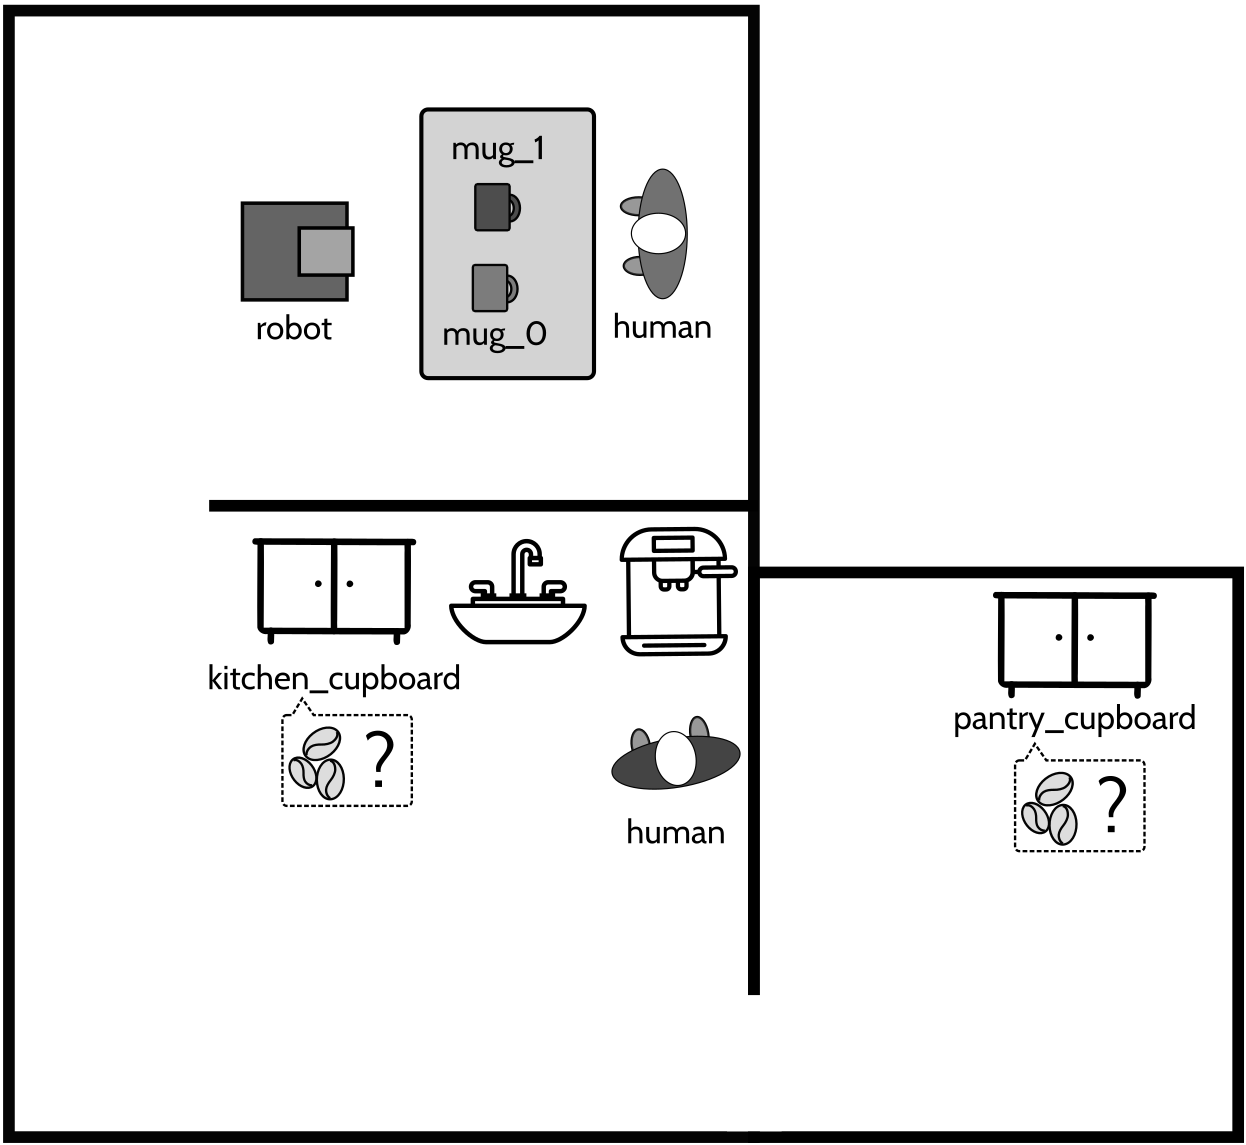
\includegraphics[width=0.9\textwidth]{figures/chapter4/Chap4CoffeeScene.png}
\caption{An example scenario where the robot is requested by a worker to bring her a coffee. It must first take her mug, then go to the coffee machine, fill it with water and coffee grounds and finally fill the mug with coffee.}
\label{fig:chap4coffeescene}
\end{figure}
% Triggers vs. explicit communication
%Human asks for the robot to get a coffee. Two mugs nearby, two possible decomposition for the robot : ask for which one to take or take one. One adds "answers" to the human -> two possibilities 
\subsection{Plan for Robot Unknown Human Knowledge}
First of all, after the robot has been commanded by the worker to bring her a coffee, it must pick her mug. We want to illustrate how we can represent human knowledge that is unknown to the robot (but with a small number of possibilities), and how the planner can elaborate different plans depending on action costs and the number of possibilities. To do so, we place the robot in a scenario where the worker and it are face to face when she asks it for a coffee. There is a table between them and $n \in \intset$ mugs are placed on it. Only one mug belongs to the worker, the robot knows she knows which one it is ($\humanmodel$) but the robot does not know it ($\robotmodel$). The goal of the robot is thus to take the right mug, and to go to the coffee machine. The general idea is that we want the robot to have two ways of grabbing the right mug. Either it can take a random one, and if the human is not protesting, the robot can proceed with the rest of the task, else it tries again while knowing this mug was not the right one; or the robot can ask the human for the right mug and take it. However, as specifying the right mug through verbal communication can be costly for the human (\textit{e.g.}~highly resembling mugs, a noisy environment), asking her might not always be feasible not be the optimal solution.

\begin{figure}[hbtp]
\centering
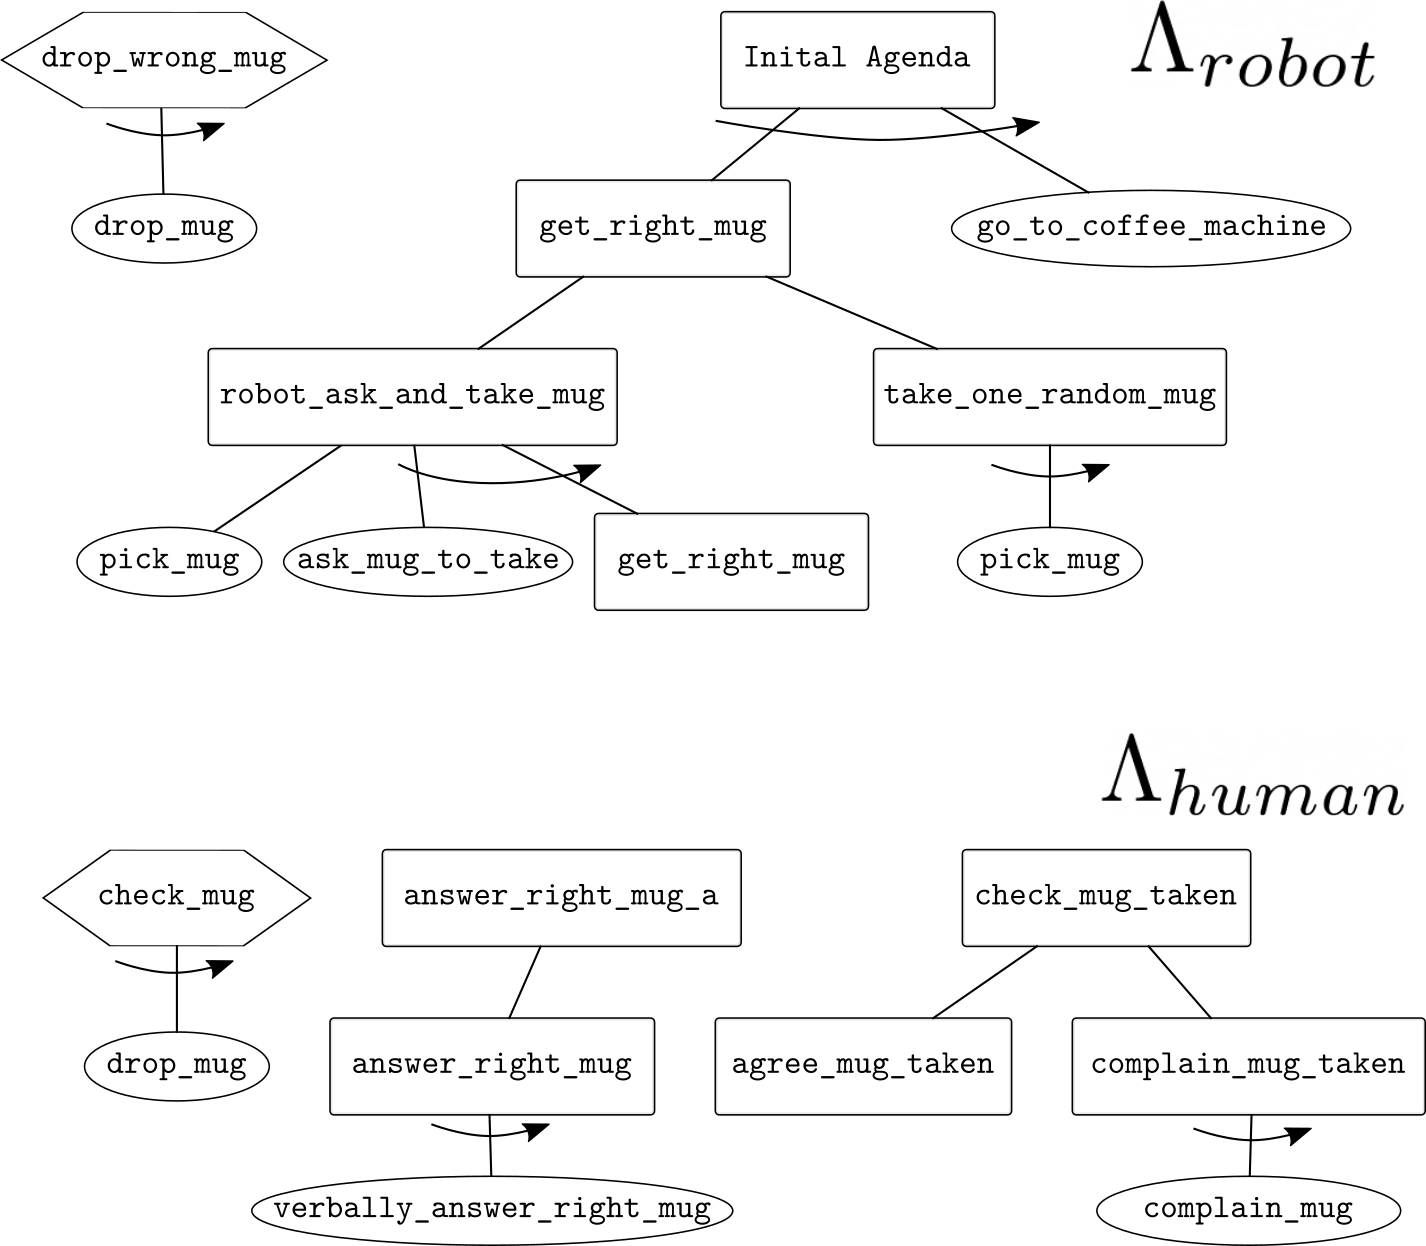
\includegraphics[width=\textwidth]{figures/chapter4/HTN_hr_mugs.png}
\caption{The action models (HTNs) of the robot and the human for the mug selection task. Rectangles represent abstract tasks, ellipses represent primitive tasks and hexagons represent triggers. The links with an arrow are ``and'' links, the others are ``or'' links. Please note that some decompositions have been merged for clarity.}
\label{fig:chap4rhhtnmug}
\end{figure}

First, we go through the design of the robot \acrshort{htn} (Figure~\ref{fig:chap4rhhtnmug}). The complete domain in Python code is presented as supplementary material in Annex~\ref{annex:domainmugs}. The robot agenda is initialized with two tasks \verb'get_right_mug' and \verb'go_to_coffee_machine'. The robot abstract tasks and their decompositions are presented here:
\begin{itemize}
\item \verb'get_right_mug' aims at making the robot pick the mug belonging to the human. It has two decompositions:
	\begin{itemize}
	\item \verb'robot_ask_and_take_mug' representing the robot asking the human which one is her mug. It returns either \verb'pick_mug' if the human's mug is known or \verb'ask_mug_to_take' and \verb'get_right_mug'
	\item \verb'take_one_random_mug' representing the robot go through trial and errors. It returns either \verb'pick_mug' if the human's mug is known or \verb'pick_mug' with all the mugs potentially belonging to the human.
	\end{itemize}
\end{itemize}
The primitive tasks (operators) of the robot and their effects are presented here:
\begin{itemize}
\item \verb'pick_mug' updating the beliefs of all the agents in the room by removing the mug given as parameter from the table and adding it to the robot gripper.
\item \verb'ask_mug_to_take' adding the task \verb'answer_right_mug_a' to the human agenda.
\item \verb'drop_mug' updating the beliefs of all the agents in the room by removing the mug they believe the robot is currently holding and adding it on top of the table.
\item \verb'go_to_coffee_machine' updating the beliefs of all agents in the room that the robot has left the room and is now in the coffee room. Moreover it updates all agents in the coffee room beliefs such as the robot is in the coffee room and updates their beliefs of what it is carrying.
\end{itemize}
Moreover, if the human is complaining about the mug the robot is currently holding, we want the robot to drop it, and to know that this mug is not the right one. To do so, we use the triggers mechanisms and we define a trigger function for the robot:
\begin{itemize}
\item \verb'drop_wrong_mug' checking if the human just complained about the mug we taken (\verb'complain_mug'~$\in \plan_h$) and if so, adds \verb'drop_mug' and \verb'get_right_mug' to the robot agenda.
\end{itemize}

Then, we go through the human task model. We assume the order of getting a coffee has already been given to the robot, and thus assume the human has no task to decompose initially in her agenda. When asked for which mug belongs to her, we model that she can answer whatever mug she has not ruled out. Moreover, we model that when the robot picks a mug, she will complain if it is not the right one. Here are the two abstract tasks and their decompositions we used to model this human behavior:
\begin{itemize}
\item \verb'answer_right_mug_a' representing the task of answering the robot for the right mug. For this example, it has only one decomposition:
	\begin{itemize}
	\item \verb'answer_right_mug' if the right mug is present in the human beliefs, it returns only the \verb'verbally_answer_right_mug' primitive task, else, it returns $m \in \intset$ alternatives of \verb'verbally_answer_right_mug' with $m$ being the number of mug not having been ruled out in the plan at this state.
	\end{itemize}
\item \verb'check_mug_taken' models the human expectation of the robot taking the right mug. It has two decompositions:
	\begin{itemize}
	\item \verb'agree_mug_taken' when the robot has the right mug in its gripper. It always returns an empty task list.
	\item \verb'complain_mug_taken' when the robot has a wrong mug in its gripper. It return the primitive task \verb'complain_mug'.
	\end{itemize}
\end{itemize}
The following presents the modeled human primitive tasks:
\begin{itemize}
\item \verb'verbally_answer_right_mug' updating the beliefs of all the agents in the room with the human being the owner of the mug passed as a parameter. To estimate the feasibility and the cost of this action we run our \acrshort{reg} component as detailed in the previous chapter. 
\item \verb'complain_mug' updating the beliefs of all the agents in the room with the human not being the owner of the mug passed as parameter.
\end{itemize}
Finally, to model the human reaction when the robot grabs the wrong mug, we use the triggers system for the human:
\begin{itemize}
\item \verb'check_mug' adding the task \verb'check_mug_taken' to the human agenda each time the robot takes a mug that has not been specially designated by the human (\textit{i.e.}~the robot has a mug in its gripper and \verb'verbally_answer_right_mug'~$\notin \plan_h$).
\end{itemize}

Another way of representing the human reaction is to represent the shared goal of the human and the robot (as the human just asked the robot to perform a task) by adding a monitoring task to the human agenda in the initial state. This monitoring task could then be refined into a \textit{WAIT} or into a \verb'complain_mug' or an empty task list depending on the mug taken by the robot. Such a representation allows to model the joint activity between the human and the robot. However, it also models that the human can do nothing else except monitor the robot actions until it has picked the right mug. Using the triggers as presented here, allows to represent that the human is maybe performing another task (modeled by the $IDLE$) action and is not committed to interact with the robot. The triggers still present a drawback in this case, as it would be triggered whenever the robot is picking a mug (provided that the human is estimated to see the action), even if it is not for serving the human. It is not an issue in the presented example as the task is quite short, but we still have to find ways to provide more context to the triggers. An easy solution would be to add a fact to the human beliefs enabling or not the trigger. We are currently investigating how to represent complex shared goals, and think they can be an answer to this issue. 



\begin{figure}[hbtp]
\centering
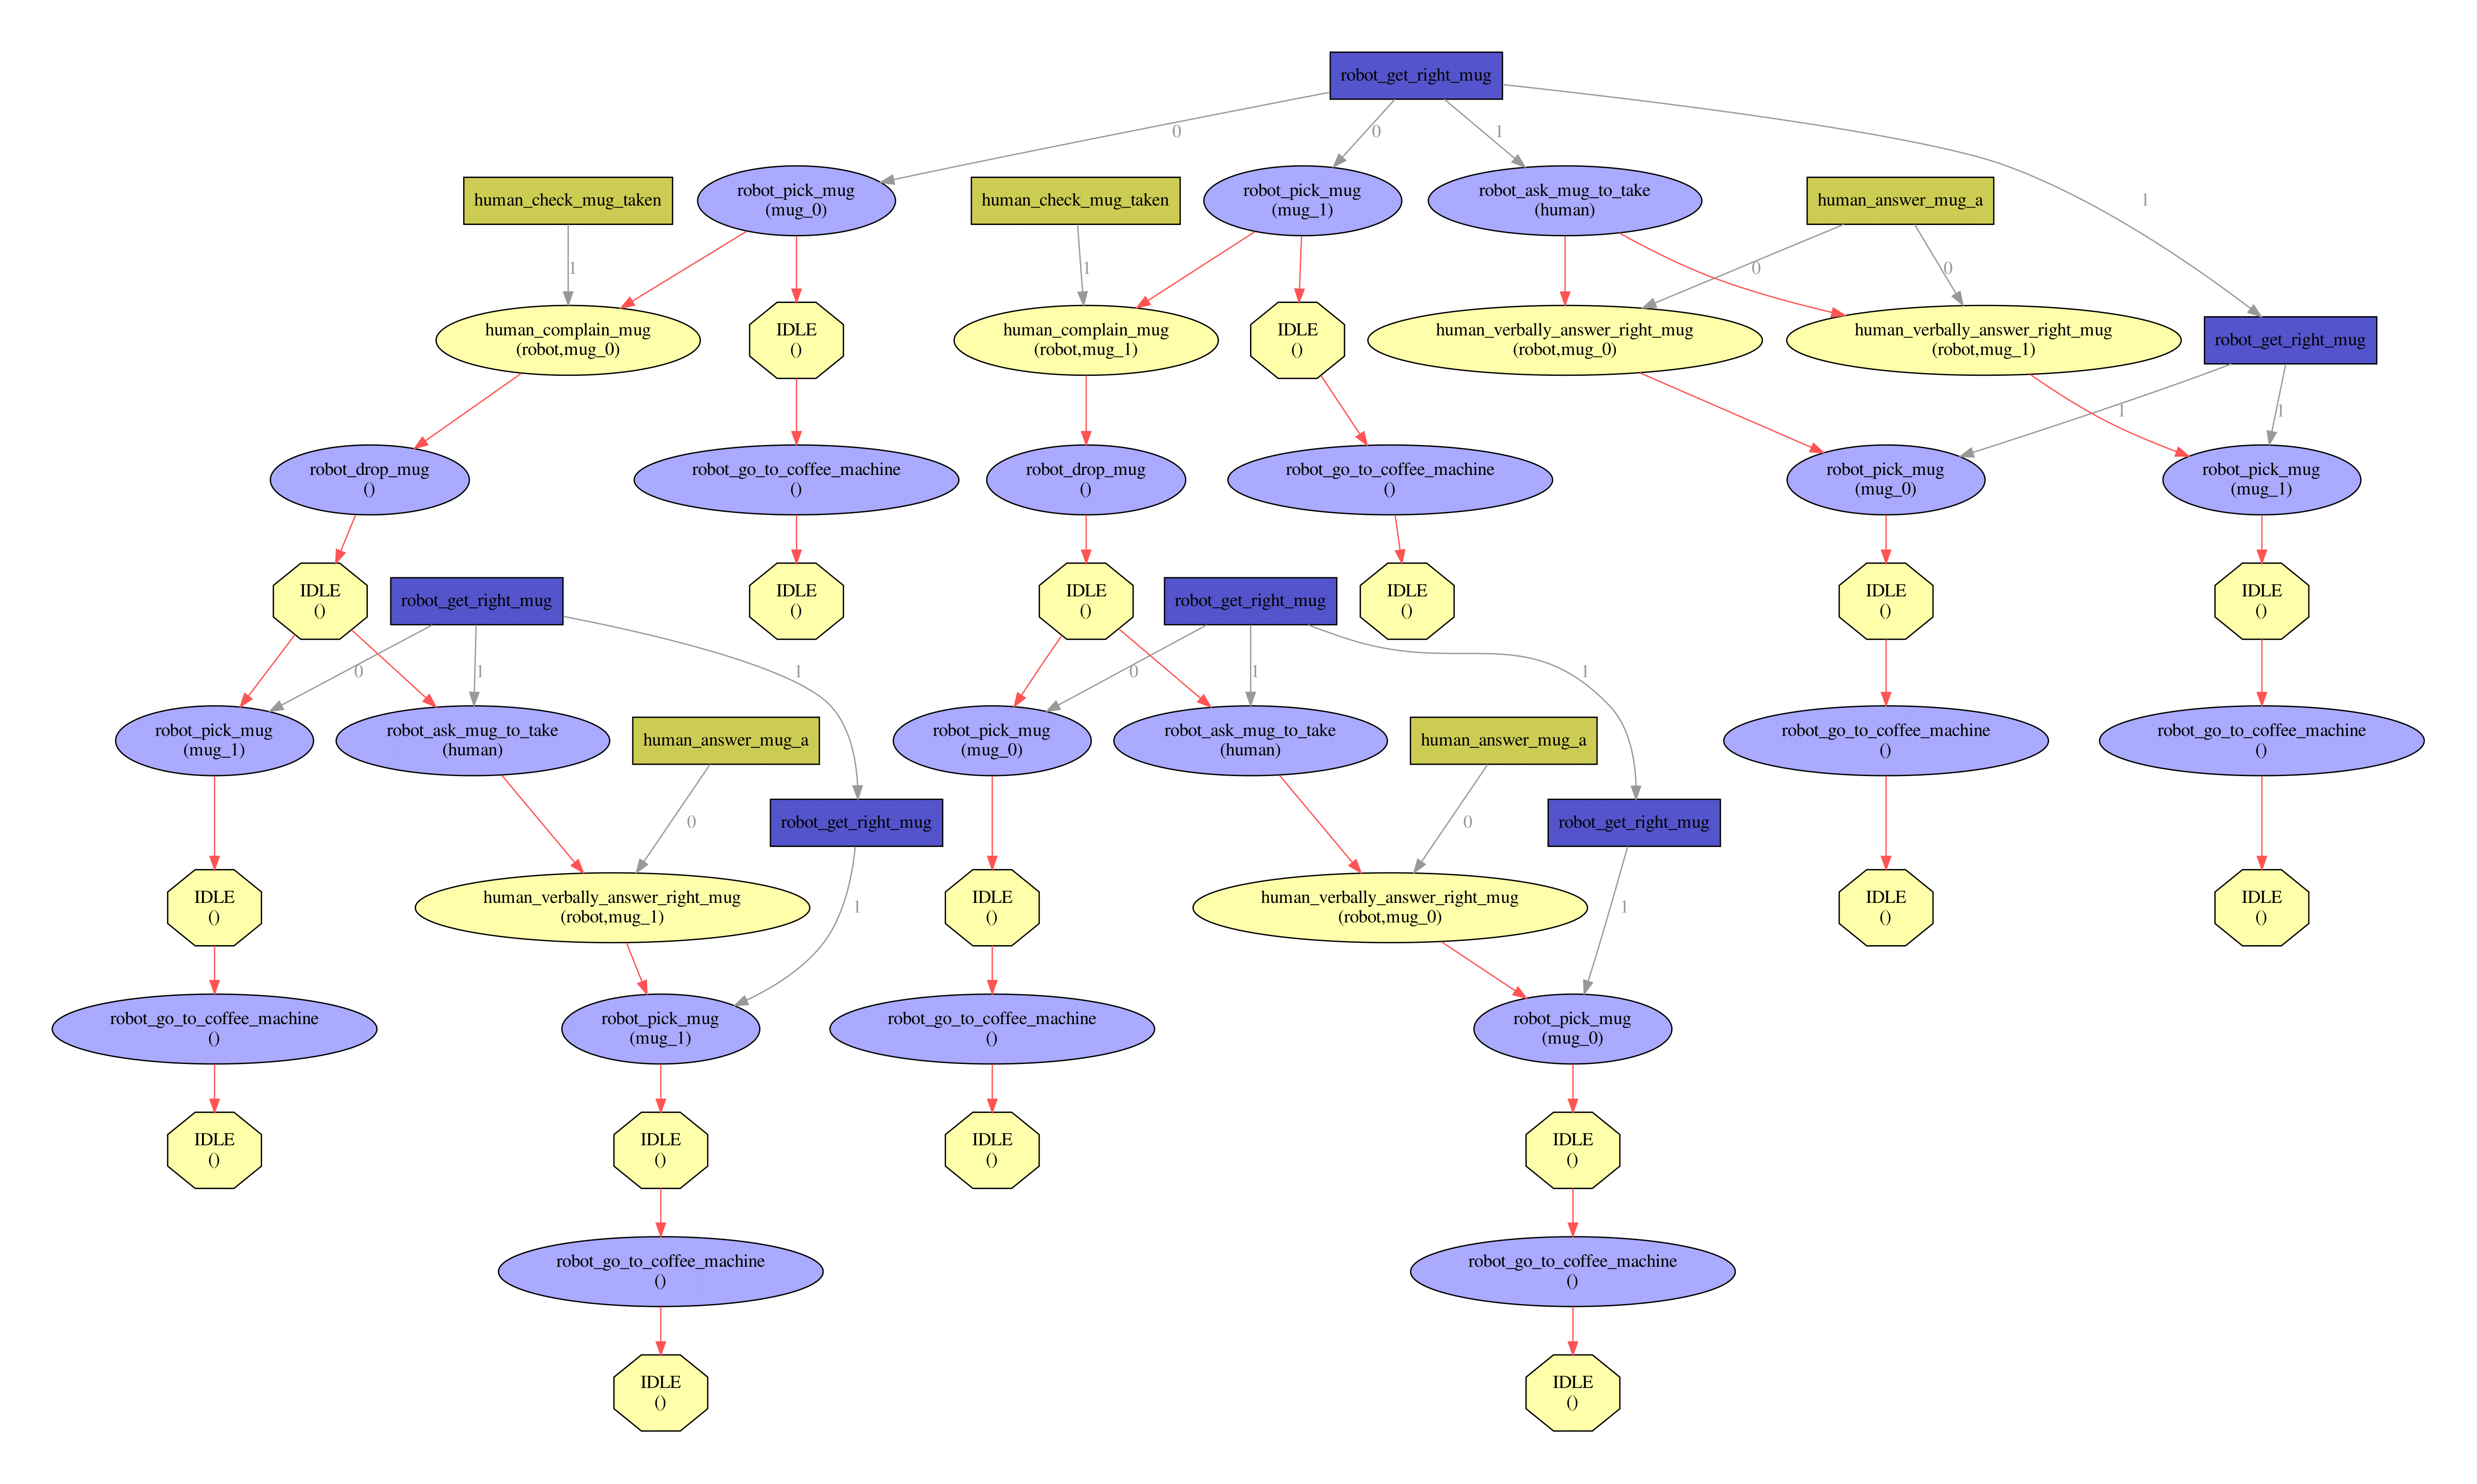
\includegraphics[height=\textwidth,angle=90,origin=c]{figures/chapter4/mug_selection_search_space.png}
\caption{The valid plans tree produced after the exploration of the HTNs.}
\label{fig:chap4mugsss}
\end{figure}

The search space for $n=2$ mugs is presented in Figure~\ref{fig:chap4mugsss}. In this example, both mugs are distinct and RE can be computed. On the right hand side of the figure is the decomposition where the robot explicitly asks the human to designate her mug. The answer can either be \verb'mug_0' or \verb'mug_1'. The robot then picks the right one and goes to the coffee machine, leaving no task to decompose.
On the left hand side of the figure is the decomposition where the robot proceeds via trials and errors. The robot can either pick \verb'mug_0' or \verb'mug_1' and the human will either react by doing nothing (if the robot took the right mug) or by complaining, in which case the robot will drop the mug, take the other one, and leave. Interestingly, we model the human reaction such as not expecting her to complain when taking the second mug after a first failure (in Figure~\ref{fig:chap4mugsss}, the only modeled returned human action after the \verb'pick_mug' actions denoted (a) and (b) is \verb'IDLE' and there are no \verb'complain_mug_taken' action as the other mug as been excluded before in this branch, so we assume that the last one is the right one).

Next, we will compare different action costs and conditional plan selection criteria based on the same search space. To select a plan we used the Algorithm~\ref{alg:minaverage}. First, we set the cost of \verb'complain_mug' action much lower than the \verb'verbally_answer_right_mug' action. Here, the costs might have been set by the supervision component, estimating we are interacting in a noisy environment, where verbal communications are difficult to make, or that the human does not bother to correct the robot. The conditional plan returned is presented in Figure~\ref{fig:chap4mugtrialerror}. The chosen plan is the one containing trials and errors. Indeed, as it can lead to much shorter and thus less costly plans, it is the minimum average. 

\begin{figure}[hbtp]
\centering
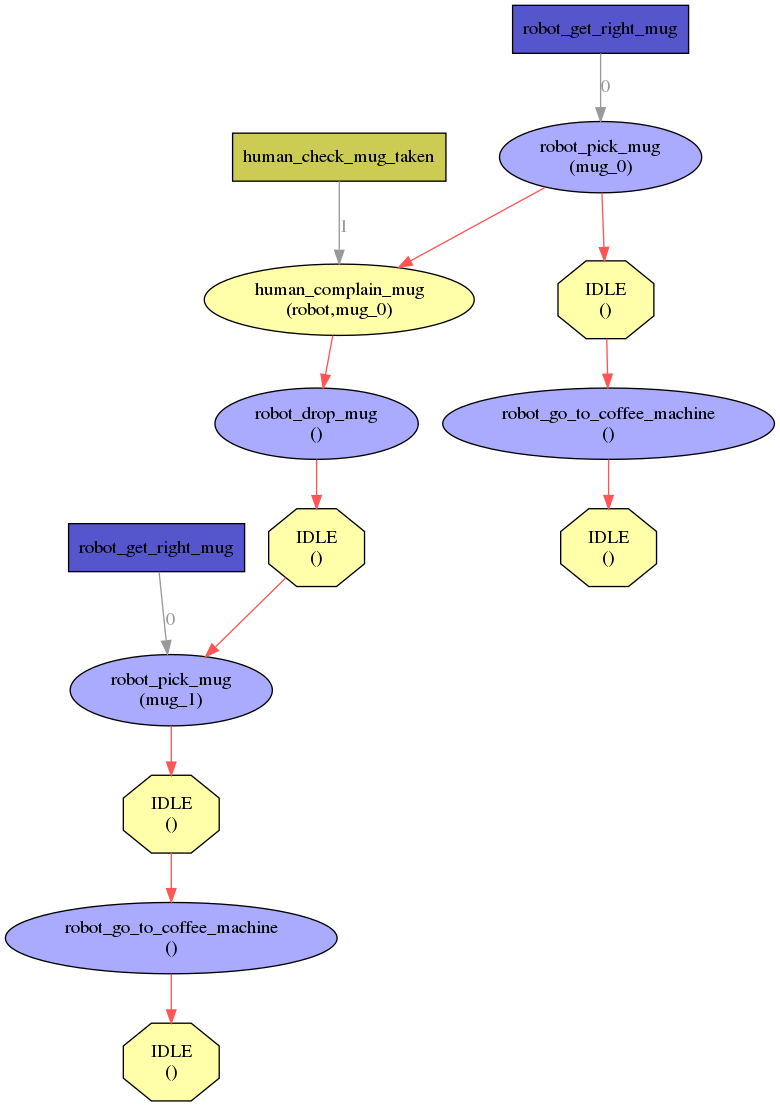
\includegraphics[width=0.9\textwidth]{figures/chapter4/mug_selection_trials.png}
\caption{A conditional plan selected from the tree depicted in Figure~\ref{fig:chap4mugsss}. In this plan, the robot starts by picking the \texttt{mug\_0} and expects the human to either complain that it is not her mug or do nothing allowing the robot to leave. If it is not the right mug, the robot would take the other one before leaving the room.}
\label{fig:chap4mugtrialerror}
\end{figure}

However, imagine that the human (who has still not had her coffee) is in a hurry, or that the mugs are really easy to distinguish from one another (\textit{e.g.}~different color) and thus, we decrease the cost of the \verb'verbally_answer_right_mug' action and increase the cost of the \verb'complain_mug' action. The conditional plan selected is presented in Figure~\ref{fig:chap4mugask}. The robot now prefers to ask for the right mug rather than trying to pick one at random.

\begin{figure}[hbtp]
\centering
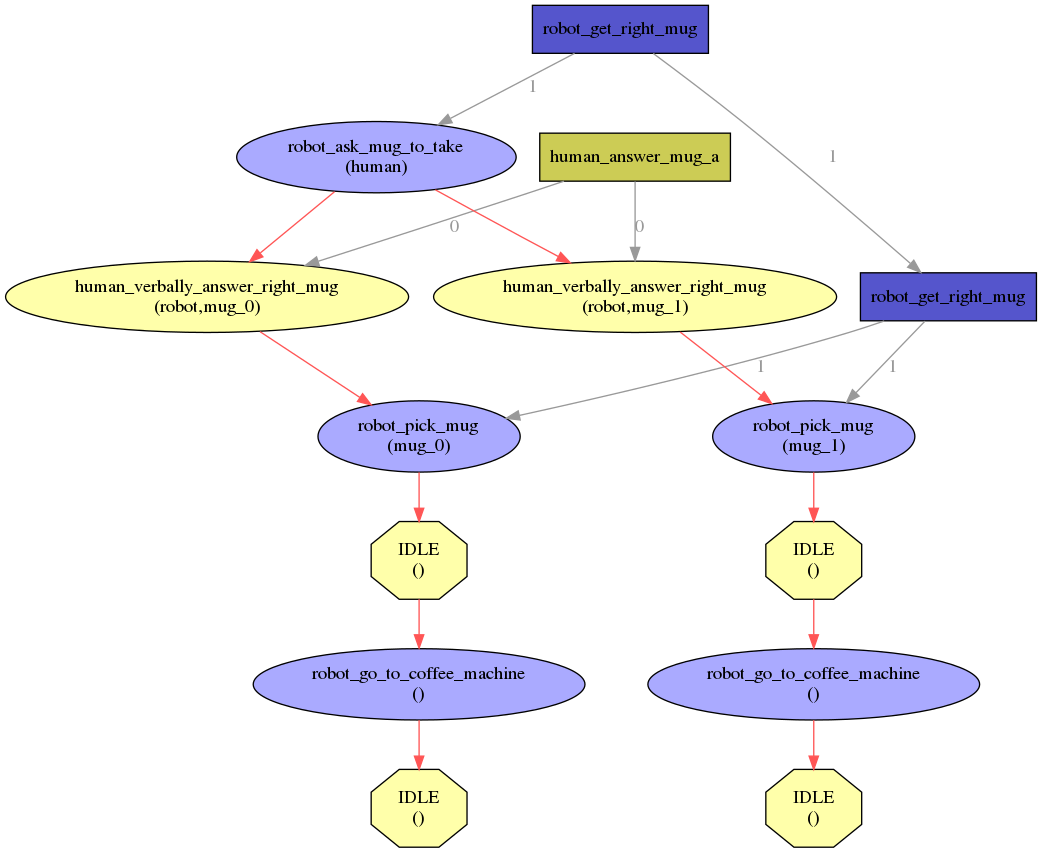
\includegraphics[width=\textwidth]{figures/chapter4/mug_selection_ask.png}
\caption{Another conditional plan selected from the tree depicted in Figure~\ref{fig:chap4mugsss}. In this plan, the robot starts by asking which mug belongs to the human. Depending on the answer, the robot would then pick one or the other and leave the room.}
\label{fig:chap4mugask}
\end{figure}

As we increase the number of mugs $n$, the cost of \verb'verbally_answer_right_mug' has to also increase to make the robot choose the trials and errors decomposition, as the average of this decomposition increases since the number of potential errors increases. 
%Finally, if we make two mugs for which the REG does not find any solution (the mugs are not distinguishable from one another) the planner is able to generate conditional plans where it first tries to <-- not true for now, as we do not take into account failed actions in cost computation....
\begin{table}[htb]
\centering
\resizebox{\textwidth}{!}{%
\begin{tabular}{c||c|c|c|}
\textbf{Number of mugs} & \textbf{\begin{tabular}[c]{@{}c@{}}Number of\\explored branches\end{tabular}} & \textbf{\begin{tabular}[c]{@{}c@{}}Duration of\\the exploration step (s)\end{tabular}} & \textbf{\begin{tabular}[c]{@{}c@{}}Duration of\\the plan selection step (s)\end{tabular}} \\ \hline
\textbf{1}              & 2                                    & 0.010                         & <0.001                           \\
\textbf{2}              & 8                                    & 0.115                         & 0.003                            \\
\textbf{3}              & 30                                   & 1.162                         & 0.006                            \\
\textbf{4}              & 128                                  & 26.425                        & 0.035                            \\
\textbf{5}              & 650                                  &                               987.057                       & 0.149                                 
\end{tabular}%
}
\caption{Planning computation durations depending on the specified number of mugs on the table.}
\label{tab:plannertime}
\end{table}

In this example, we show one really interesting feature of \acrshort{hatpehda}: representing human knowledge that is not known by the robot. While not being tractable when there are a lot of possibilities, which is expected when exploring all the possibilities in non-deterministic planners, it allows to select more or less conservative conditional plans depending on the cost of each action. Computational times are given in Table~\ref{tab:plannertime}. We see that this task modeling begins to fail at 4 mugs, as a large computation time will spoil the interaction. Although, we think it is still pertinent in \acrshort{hri} as we seldom deal with a large number of objects and long plans. Besides, thanks to the task decomposition being Python functions, we can make a decomposition fail if it would lead to a combinatorial explosion. Here we could have made the ``trial and error'' decomposition fails if the number of mugs was greater than 4. Moreover, this example allowed to see how updating the human agenda and how triggers can be used to model the agents interaction in the \acrshortpl{htn} planning.
However, the human model was pretty simple, and we propose to challenge \acrshort{hatpehda} in the next example with a task where the human is more involved. The complete domain in Python code is presented as supplementary material in Annex~\ref{annex:domaincoffee}.

\subsection{Balance Difficult Communications, Decomposition Cost and Task Attribution}
The robot is now heading to the coffee machine with the right mug in its gripper. On its way it detects another human taking a break near the coffee machine. The coffee has to be made. To brew coffee, ground coffee and water must be put in the coffee machine, and then the coffee can be served. While water is considered as always available, ground coffee is not. There are two places where ground coffee can be retrieved: either in the kitchen cupboard (close to the coffee machine) or in the pantry cupboard. 

\subsubsection{Handling the Robot Only Case}
\label{subsubsec:chap4coffeerobotonly}
\begin{figure}[hbtp]
\centering
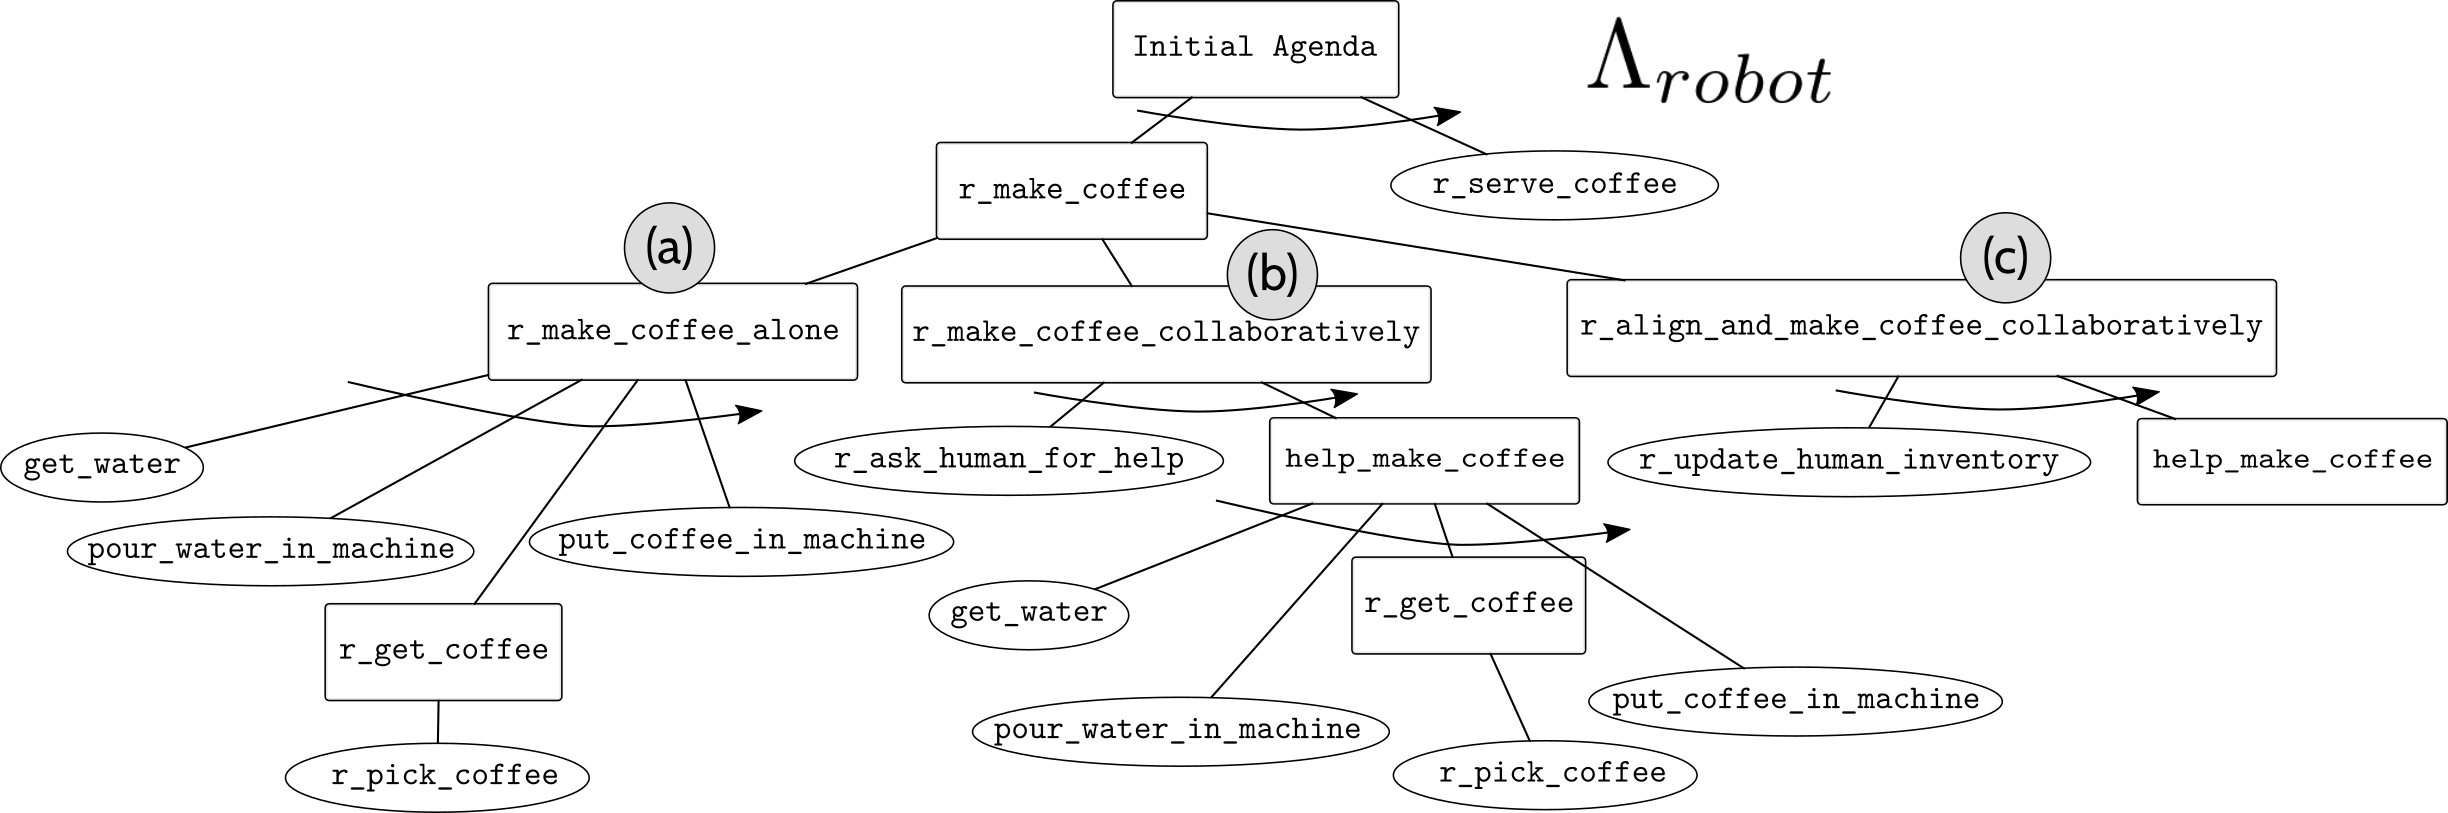
\includegraphics[height=0.47\textwidth, angle=90, origin=c]{figures/chapter4/HTN_r_coffee.png}
\caption{The action models (HTN) of the robot for the coffee preparation task. Rectangles represent abstract tasks and ellipses represent primitive tasks. The links with an arrow are ``and'' links, the others are ``or'' links. Please note that some decompositions have been merged for clarity.}
\label{fig:chap4rhtncoffee}
\end{figure}

First, we want the robot to be able to make coffee by itself, without requiring human help. To do so, we implement the following abstract tasks tree depicted in Figure~\ref{fig:chap4rhtncoffee} in the robot model (here we prepend the task names with \verb'r' where task are different in the robot and the human model):

\begin{itemize}
\item \verb'r_make_coffee' only having one decomposition (for now), represented by Figure~\ref{fig:chap4rhtncoffee}(a):
	\begin{itemize}
	\item \verb'r_make_coffee_alone' returning, in both orders (to represent partially ordered task tree), the tasks \verb'get_water', \verb'pour_water_in_machine' and \verb'r_get_coffee', \verb'put_coffee_in_machine'. Only \verb'r_get_coffee' is an abstract task.
	\end{itemize}
\item \verb'r_get_coffee' representing the ways for the robot to obtain coffee. It has only one decomposition:
	\begin{itemize}
	\item the decomposition returns $()$ if the robot has already coffee in its gripper. Else, it selects the closest cupboard and returns \verb'r_pick_coffee' with it as parameter.
	\end{itemize}
\end{itemize}

The robot primitive tasks as are follow:
\begin{itemize}
\item \verb'get_water' returning $\bot$ if the robot is already holding something; updating the beliefs of all the agents in the room with the fact that the robot holds water otherwise.
\item \verb'pour_water_in_machine' updating all the agents in the room beliefs with the machine being filled with water.
\item \verb'r_pick_coffee' returning $\bot$ if the robot is already holding something or if the cupboard passed as parameter does not contains coffee (in the robot beliefs); updating the beliefs of all agents in the room with the fact the the robot holds coffee otherwise.
\item \verb'put_coffee_in_machine' updating all the agents in the room beliefs with the machine being filled with coffee.
\item \verb'r_serve_coffee' updating all the agents in the room with the mug being filled with coffee.
\end{itemize}

Now, for the initial conditions we set that the robot knows there is coffee in the kitchen cupboard (the closest) and we add two tasks in its agenda: \verb'r_make_coffee' and \verb'r_serve_coffee'. The human has nothing in its agenda. The two possible plans for this really simple case are presented in Figure~\ref{fig:chap4coffeesimplerobotonly}(a) and (b). The plan selection would then choose one of the plans based on robot action costs.

This simple example shows that our approach can still be used as a classical \acrshort{htn} planner and that it can plan for partially ordered task networks. By doing so, we show the planner does not require to always involve the human and can balance joint plans with plans where it does all the task when applicable.

\begin{figure}[hbtp]
\centering
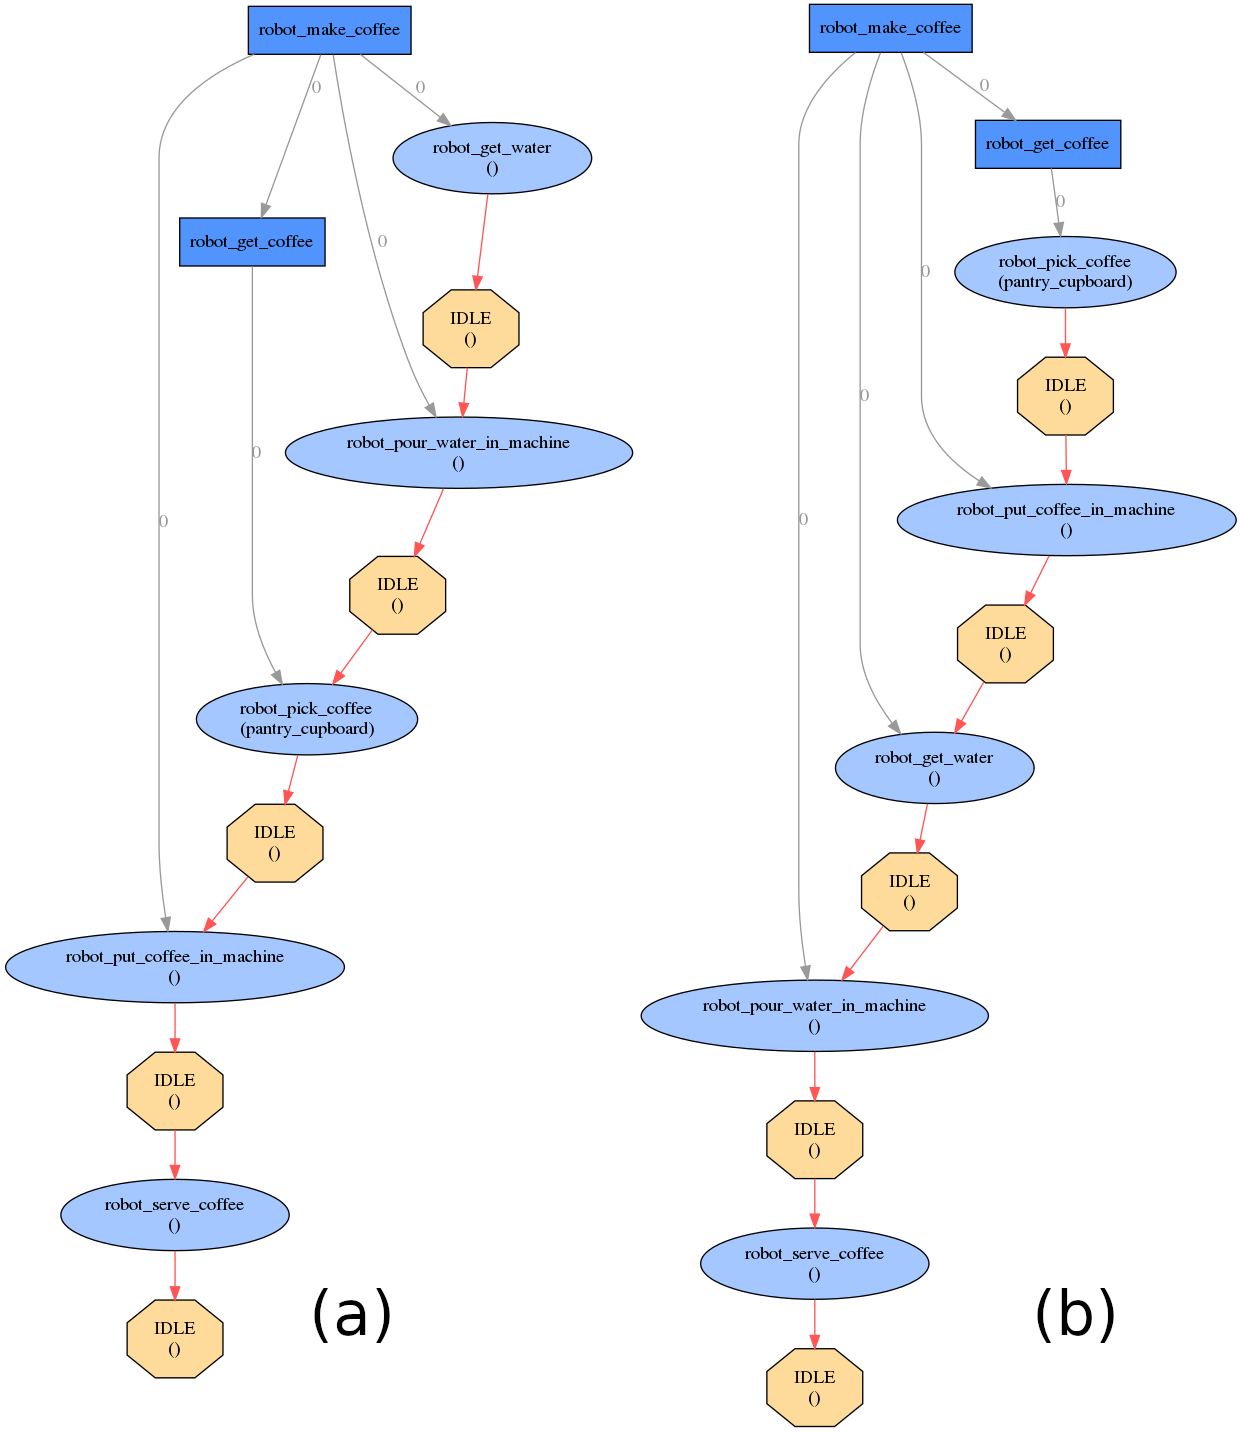
\includegraphics[width=\textwidth]{figures/chapter4/Chapt4SimplePlanHierarchy.png}
\caption{The conditional plans generated by our approach. In both (a) and (b) the robot chooses not to involve the human and do the coffee on its own, only the order of action changes.}
\label{fig:chap4coffeesimplerobotonly}
\end{figure}

\begin{figure}[hbtp]
\centering
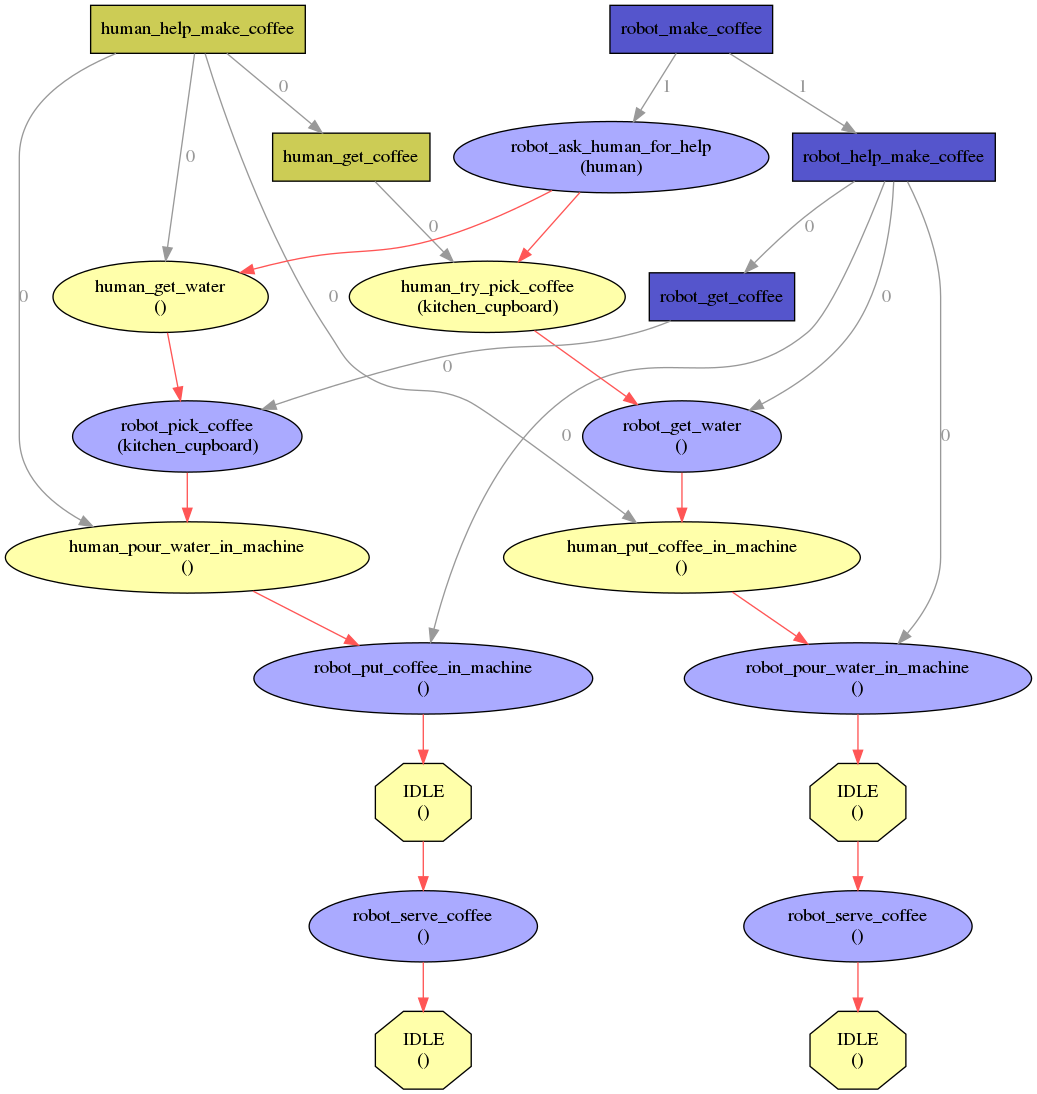
\includegraphics[width=\textwidth]{figures/chapter4/Chap4CoopNoDivergence.png}
\caption{The conditional plan involving the human selected by \acrshort{hatpehda}. The robot chooses to ask for human help. We plan that the human will either get the coffee or fill the water and adapt accordingly, the choice of human actions is not made, but thanks to the conditional plan, both possible solutions are planned and it is up to the supervision component to follow the right one depending on the human action detected during execution.}
\label{fig:chap4coffeecoopnodivergence}
\end{figure}


\subsubsection{Incorporating the Human Planning Process}
As we also want the robot to be able to ask the idle human to help it, we add, to its action model, a decomposition to the abstract task \verb'r_make_coffee' and a new abstract task \verb'help_make_coffee':

\begin{itemize}
\item \verb'r_make_coffee' containing the previous decomposition and the new one, represented in Figure~\ref{fig:chap4rhtncoffee}(b):
	\begin{itemize}
	\item \verb'r_make_coffee_collaboratively' returning a sequence containing the primitive task \verb'r_ask_human_for_help' and the abstract task \verb'help_make_coffee'
	\end{itemize}
\item \verb'help_make_coffee' representing the ways for the robot to help another agent to make coffee. It has only one decomposition:
	\begin{itemize}
	\item It returns \verb'get_water' and \verb'pour_water_in_machine' if there is no water in the machine (in $\worldstate_{robot}$) and the human is doing a task related to bringing coffee (in $\agenda_{human}$). Likewise, it returns \verb'r_get_coffee' and \verb'put_coffee_in_machine' if there is no coffee in the machine (in $\worldstate_{robot}$) and the human is doing a task related to fill the machine with water (in $\agenda_{human}$). Then, if the human is not doing any task (in $\agenda_{human}$), we add to the exploration \verb'r_get_coffee', \verb'put_coffee_in_machine' and \verb'help_make_coffee' if there is no coffee in the machine (in $\worldstate_{robot}$) and \verb'get_water', \verb'pour_water_in_machine' and \verb'help_make_coffee' if there is no water in the coffee machine (in $\worldstate_{robot}$). The idea here is to complete the human actions if they take the initiative of a task, but to be proactive by exploring both possible alternatives if they are not. The recursion allows to reevaluate the need for this task later in the planning process.
	\end{itemize}
\end{itemize}

The primitive action added to the robot model is:
\begin{itemize}
\item \verb'r_ask_human_for_help' adding the task \verb'help_make_coffee' to the human agenda. Here we could have represented the possible refusal of the human by adding an abstract task leading to two possible decompositions for the human, accepting or declining, leading in similar schemes as in \ref{subsubsec:chap4coffeerobotonly}. However, to keep this example as simple as possible, we assume the human will always help the robot if asked to do so.
\end{itemize}

\begin{figure}[hbtp]
\centering
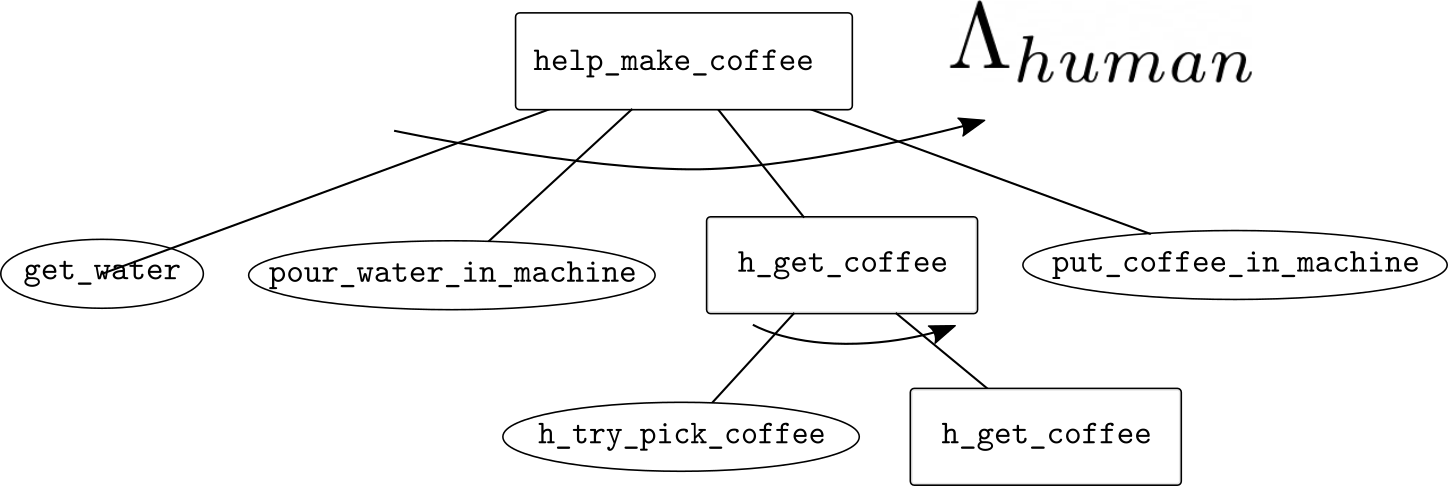
\includegraphics[width=\textwidth]{figures/chapter4/HTN_h_coffee.png}
\caption{The action models (HTN) of the human for the coffee preparation task. Rectangles represent abstract tasks and ellipses represent primitive tasks. The links with an arrow are ``and'' links, the others are ``or'' links. Please note that some decompositions have been merged for clarity.}
\label{fig:chap4hhtncoffee}
\end{figure}

We model the human actions similarly to the robot ones. Their abstract tasks are represented in Figure~\ref{fig:chap4hhtncoffee} and defined as:
\begin{itemize}
\item \verb'help_make_coffee' representing the ways for the human to help another agent to make coffee. It has only one decomposition, which is the same as the robot one.
\item \verb'h_get_coffee' representing the ways for the human to obtain coffee. It has only one decomposition:
	\begin{itemize}
	\item the decomposition returns $()$ if the human is already holding coffee (in $\worldstate_{human}$). Else, it selects the closest cupboard and returns \verb'h_try_pick_coffee' with it as parameter and \verb'h_get_coffee'. It differs from the robot one, indeed, whereas the knowledge of the robot is assumed to be the world state, the human's one can be false. Thus, the human might try to perform \verb'h_try_pick_coffee' on a cupboard not containing coffee. We take this into account with the recursion of this abstract task, and with the primitive task \verb'h_try_pick_coffee' described hereafter.
	\end{itemize}
\end{itemize}

The model of the human primitive tasks are:
\begin{itemize}
\item \verb'get_water' as defined for the robot
\item \verb'pour_water_in_machine' as defined for the robot
\item \verb'h_try_pick_coffee' differs from the one defined for the robot as it checks if the cupboard passed as parameter really contains coffee (\textit{i.e.}~in the robot beliefs $\worldstate_{robot}$). If it does not, the human's beliefs ($\worldstate_{human}$) about this cupboard are updated to match the robot ones ($\worldstate_{robot}$, modeling the human going in front of the cupboard, opening it and seeing the absence of coffee). If the cupboard does contain coffee in the robot beliefs, all the agents in the room beliefs are updated with the human having coffee in their hand.
\item \verb'put_coffee_in_machine' as defined for the robot.
\end{itemize}

The initial conditions are the same as presented before, but we also add that the kitchen cupboard contains coffee in the human beliefs. In addition to the two plans where the robot does not seek human help (Figure~\ref{fig:chap4coffeesimplerobotonly}(a) and (b)), another valid plan is found. This plan is presented in Figure~\ref{fig:chap4coffeecoopnodivergence}. This conditional plan has two alternatives, depending on the initiative taken by the human.

Moreover, we see how recursive abstract tasks are used to reevaluate the agents state later in the plan to adapt for the other agent planned actions. However, recursions in abstract tasks usually break the semantic of the returned plan hierarchy and can prevent (or alter) their communication or storage. We envision in the future to allow to flag some abstract tasks as iterative to decouple their exploration from the returned plan hierarchy.

The planner is then able to balance between asking the human to take part in the task (Figure~\ref{fig:chap4coffeecoopnodivergence}) or doing it all on its own (Figure~\ref{fig:chap4coffeesimplerobotonly}(a) and (b)). Creating a shared goal or engaging in a joint action now depends on the costs set and is decided by the planner. Moreover, we chose to not impose a specific task to the human (either fetching the coffee or filling the water) but to give a high level shared goal of making coffee. We thus rely on the human planning capabilities to perform the actions. Besides, the human has the initiative of the part of the shared goal he wants to perform, but thanks to conditional plans, both choices are covered and planned for. It allows to make more accurate plans and to choose between them in a more informed way as they account for multiple alternatives. Once a plan is selected, it is up to the supervision component to follow the right branch depending on the detected human action during the execution (\textit{i.e.}~for the plan represented in Figure~\ref{fig:chap4coffeecoopnodivergence} if the human is getting water from the tap, or if he is picking coffee from the cupboard).

\subsubsection{Updating Human Beliefs}
We can also change the initial conditions to elicit new behaviors. We keep the same action models for both the robot and the human, but we change the estimation of the human beliefs given as initial conditions to the planner. In a real robotic architecture, the human knowledge base would be updated with an estimation provided by situation assessment components. We specify that the human believes that both the kitchen and the pantry cupboard contain coffee ($\worldstate_{human}$). However, the robot knows (\textit{e.g.}~using specific sensors or having been told about) that there is coffee only in the pantry cupboard ($\worldstate_{robot}$). With these conditions, the search space extends from the three plans presented in Figure~\ref{fig:chap4coffeesimplerobotonly}(a), (b) being when the robot prepares the coffee by itself, to include the one presented in Figure~\ref{fig:chap4beliefsdivnoalign}. In this last plan, we indeed model that the human will tend to first go to the nearest cupboard he thinks contains coffee. If this cupboard does not contain coffee, he will go to the next one. We can also note that only the left branch of the plan in Figure~\ref{fig:chap4beliefsdivnoalign} is impacted by this beliefs divergence. However, this branch choice is not up to the robot as we modeled the human as having the initiative of selecting a task. This subtlety cannot be represented in \acrshort{hatp}. Indeed, in \acrshort{hatp}, only one task would have been assigned to the human corresponding the to optimal plan being the one where the human fills the water. However, without the communication of the plan, the human would have had no way of knowing which task is preferred.

Depending on the cost of the human being disappointed and of the actions, the plan selected can either be that the robot does all the task (Figure~\ref{fig:chap4coffeesimplerobotonly}(a) and (b)), as the human first searching in the wrong cupboard can increase too much the average cost; or the new plan (Figure~\ref{fig:chap4beliefsdivnoalign}) asking the human for help but taking the risk that he may do the coffee part and, given his beliefs, go to the wrong cupboard.

\begin{figure}[hbtp]
\centering
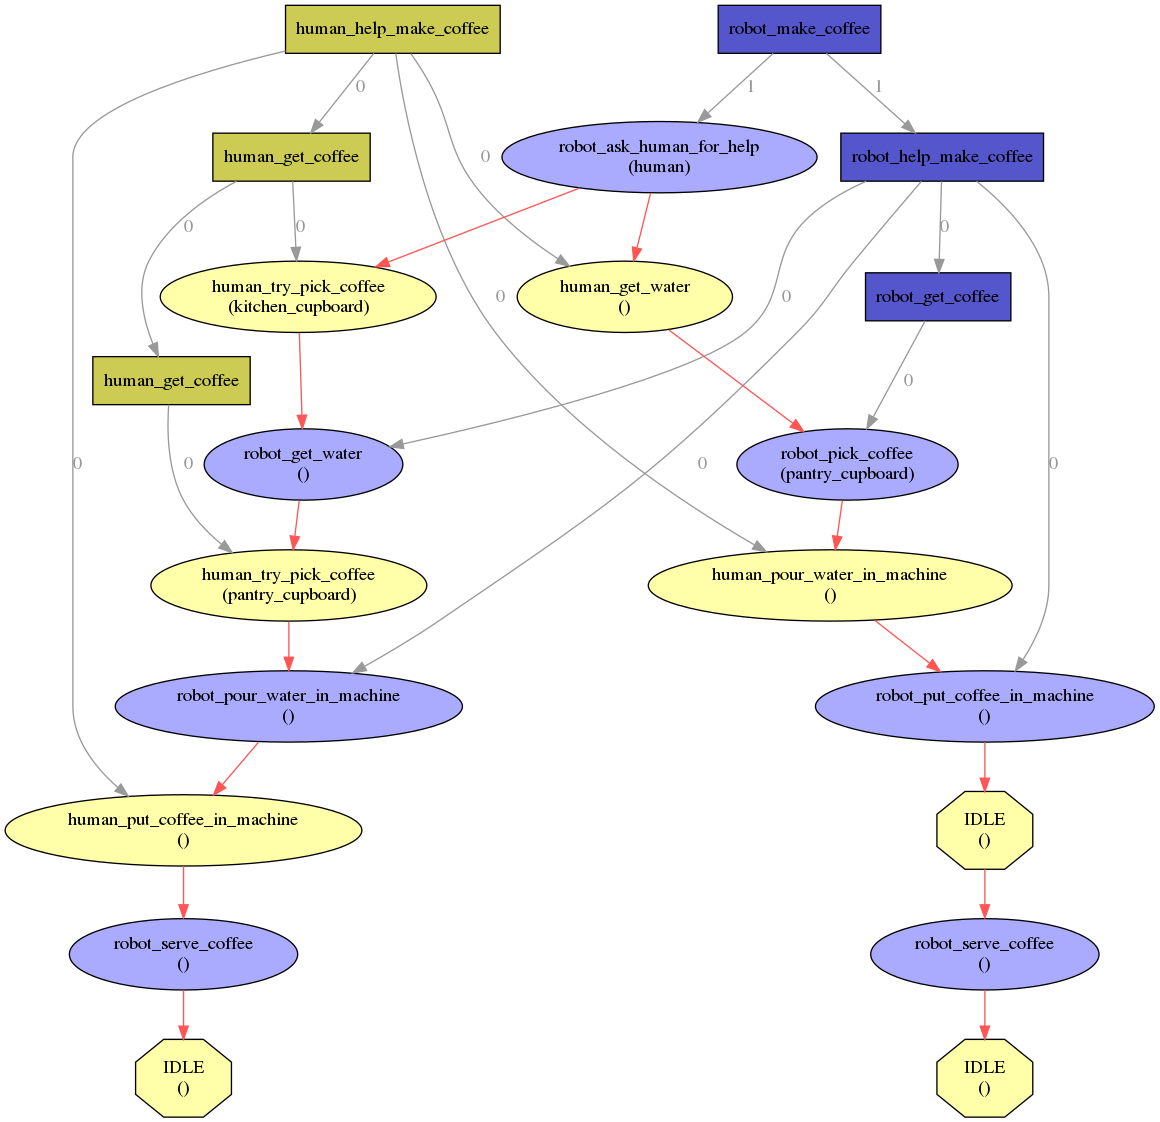
\includegraphics[width=\textwidth]{figures/chapter4/Chap4CoopDivergence.png}
\caption{A conditional plan returned by the planner to make coffee with human help in case of (known) beliefs divergence. The robot chooses to keep this divergence, potentially leading to the human erroneously opening the wrong cupboard to fetch coffee before trying the right one.}
\label{fig:chap4beliefsdivnoalign}
\end{figure}

To improve our robot, we want to make it able to realign the beliefs of the human, so, whatever the task he chooses, he will not go to the wrong cupboard. 

To do so, we add a third decomposition to the \verb'r_make_coffee' abstract task and one new primitive task to the robot models.
\begin{itemize}
\item \verb'r_make_coffee' containing the previous two decompositions and the new one, represented in Figure~\ref{fig:chap4rhtncoffee}(c):
	\begin{itemize}
	\item \verb'r_align_and_make_coffee_collaboratively' returning $\bot$ if no beliefs divergence is detected between the robot and the human. Otherwise, the decomposition returns the new primitive task \verb'r_update_human_inventory' along with \verb'r_ask_human_for_help' and \verb'r_help_make_coffee'. An alternative for \verb'r_update_human_inventory' is returned with as parameter each cupboard in diverging beliefs between the robot and the human.
	\end{itemize}
\item \verb'r_update_human_inventory' being a primitive task. It updates the human beliefs ($\worldstate_{human}$) concerning the cupboard passed as parameter with the beliefs of the robot ($\worldstate_{robot}$).
\end{itemize}

\begin{figure}[hbtp]
\centering
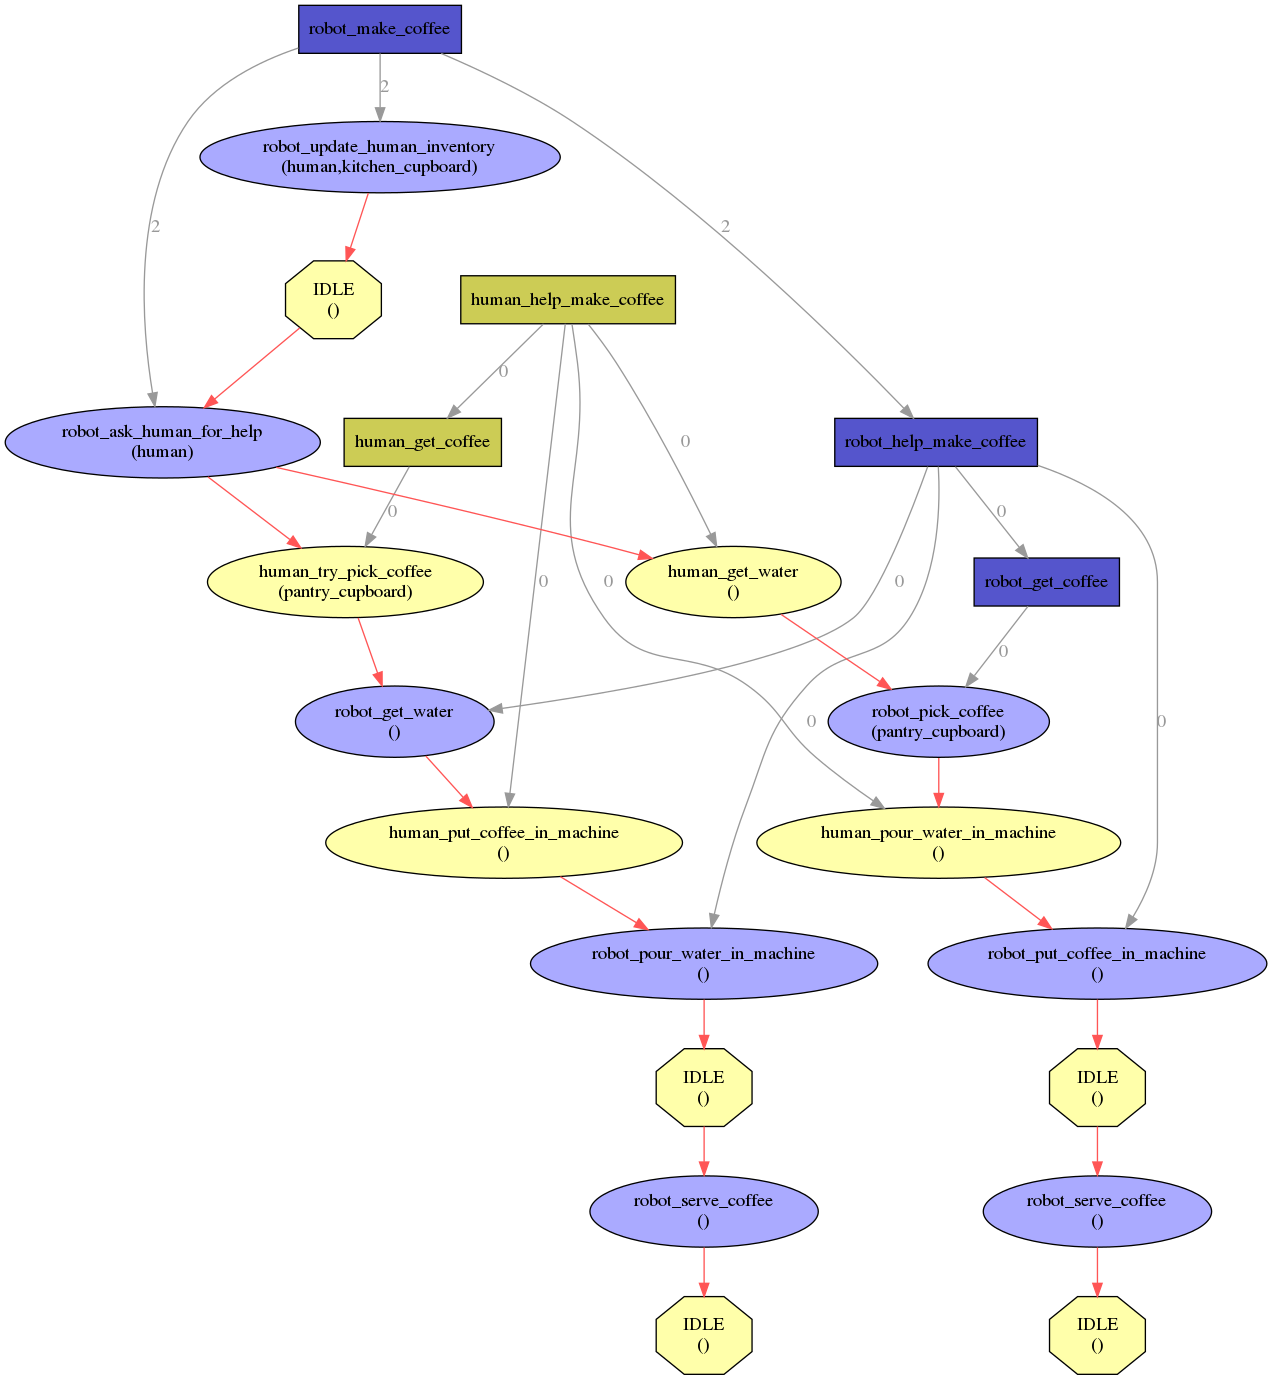
\includegraphics[width=\textwidth]{figures/chapter4/Chap4CoopRealign.png}
\caption{A conditional plan returned by the planner to make coffee with human help in case of (known) beliefs divergence. Here, the robot chooses to communicate to realign the beliefs with the human, then asking him for help, preventing any human misleading.}
\label{fig:chap4beliefsdivwithalign}
\end{figure}

In this example, we see how representing separately the agents beliefs allows to plan for communication actions helping human decision and hopefully avoiding their disappointment (increasing their satisfaction). Our planning scheme allows to plan for communication actions aligning the beliefs, thanks to the rich operator model (as Python functions) presented before. Not discovering the need of aligning the beliefs during the execution allows to include the cost (or even the feasibility) of such communication during the planning process and thus to balance with other plans not needed them.

With this new decomposition, the new plan presented in Figure~\ref{fig:chap4beliefsdivwithalign} is added to the search space. In this plan, the human beliefs are updated before asking him to help the robot to make coffee. The human does not make the first failure of going first to the kitchen cupboard to take the coffee.

Depending on the communication cost (estimated using the \acrshort{reg} approach presented in the previous chapter to designate the cupboards), the human disappointment cost (which can be added as a social cost) and the other actions cost, any one of the four possible plans can be selected. For example, to minimize the human involvement and if the communication has a high cost, the selected plan would be Figure~\ref{fig:chap4coffeesimplerobotonly}(a) or (b). If the communication is costly but the pantry and kitchen cupboard are not too far away, the selected plan is Figure~\ref{fig:chap4beliefsdivnoalign}, finally, if we represent that the human would be upset if he makes an erroneous action or if the communication for aligning beliefs is not expensive, the plan Figure~\ref{fig:chap4beliefsdivwithalign} would be returned.
Indeed, the planner may choose to leave the human with their false beliefs as it finds that it does not prevent to successfully perform the task. 

Through all these examples we show that this task planning approach, which separates human and robot beliefs and action models, can be suitable for multiple problems. We are able to plan for robot unknown human beliefs, to rely on the human planning process while keeping inherent uncertainties (\textit{i.e.}~not making choices for them, without communicating them) and also to plan diverging beliefs and balance the actions of realigning them with plans containing mistakes. In the next chapter, we present a \acrshort{hri} task, inspired from psychology, that has never been tackled in robotics and we show how \acrshort{hatpehda} is integrated into a fully functional robotic architecture dedicated for this task.

\section{Conclusion and Future Work}
In this chapter, we have proposed a new task planning approach for human robot interaction. This approach not only explicitly represents and plan upon both the human and the robot beliefs but also use two separate action models as \acrshortpl{htn} for the human and the robot.

We proposed a formalism along with an algorithm allowing to plan for robot actions, while considering the possible human actions according to their task model. By doing so, we are able to represent and to account for the human planning and reaction processes.

Then, we presented a successful implementation of this approach in Python called \acrfull{hatpehda} and showed the first results through two examples. These examples highlighted both the features of \acrshort{hatpehda} and the rationale behind the action models crafting. The planner is able to represent and to plan for robot unknown human knowledge, human reactions to robot actions, multiple human possible plans and intricate human robot tasks. It is also capable of balancing between communicating, letting the human perform a mistake and attributing different roles to the robot or the human.

We look forward to continuing exploring this approach, find its benefits and its limits. More importantly, we aspire at improving it, especially on the following topics.

\subsection{Selecting Conditional Plans Using the Human Model}
\label{subsec:chap4selectingplan}
We presented and implemented a method for selecting a conditional plan among the multiple possible ones, by selecting robot actions that minimize the average cost of the plan. This method intends to model the human as being cooperative but maybe not having all the information to be able to project themselves throughout the whole task, and maybe not performing the action leading to the optimal plan. However, this method is quite simple and does not reflect the full complexity of human decision process. We propose two other methods for conditional plan selection, which use even more the human model, that have yet to be implemented and tested.

\subsubsection{The Human Planning Process Modeled as a Limited Depth Planner}
First, we propose to consider the human as being able to plan a few steps ahead. Thus, instead of considering the average cost of all the possible human actions, we could set less importance to the ones failing a few steps ahead (as the human is likely to have foreseen the failure, and will probably not perform this action) and more importance to the ones leading to a smaller cost in the near future (as the human is likely to perform a greedy approach on the short horizon we model they can plan to).

To do so would require to also store the failing operators in the valid plans tree during the first exploration step. Moreover, it would require a new parameter being the depth at which the human is modeled to foresee in the plan. 

Then, when exploring the valid plans tree, if a failing operator is encountered at a depth smaller than the depth parameter, the cost of the corresponding plan would not be added to the average as we assume the human would not make an action leading to a failure that they can foresee. 

Moreover, the average can be weighted with smaller number for plans being evaluated as more costly than others at the depth specified by the parameter. It models that the human will not perform actions that they estimate to lead in costly plans.

This approach still needs refinement but is seen as a great improvement over considering only the cost average.

\subsubsection{Guiding Human Choices Towards the Least Costly Solution}
Then, we also want to add another step between the \acrshortpl{htn} exploration and the conditional plan selection being the addition of communication actions related to the plan. The general idea is to analyze the valid plans tree resulting from the \acrshortpl{htn} exploration and to insert robot communication action before some potential human actions that are leading to a plan failure or a costly plan. These communications would aim at encouraging some human decisions toward less costly plans, or to inform the human about the difference in the plan their actions will induce. To avoid unnecessary communications, the insertion can be conditional on the human prediction depth defined before. If the human can foresee the failure the communication is not needed.

Such communication can hardly be inserted in the \acrshortpl{htn} or during the \acrshortpl{htn} exploration step, as it requires having the full plan to decide whether they are needed or not. However, analyzing and inserting them during planning rather than after a plan has been selected or at the execution is interesting as it would allow to balance between keeping some uncertainty for non crucial human decisions or accepting the additional cost of these communication actions but reducing the uncertainty in human actions for plans easily risking a failure.

Finally, the decision to add or not such a communication can also depend on the trust the robot has in this human and on the estimated experience the human has in doing this specific task or in working with the robot.

\subsection{Representing Explicitly Observation Processes}
A lot of code is common between the primitive tasks not only in a planning domain but also between multiple ones. Indeed, the part where we update the beliefs of the agent performing the action, but also the ones of the other agents in the room is present in almost all the primitive actions. This commonality raises the question of the observability of actions. Indeed, even if we can assume that when an agent is planned to do an action they will be aware of its effects, and that if the human is planned to perform an action, even if it is not observable from the planned robot position, we update the beliefs of the robot (as it is emulating the human actions), it is not the case for a robot action and the update of human beliefs. We can represent is coarsely in the primitive task effects by relying on heuristics such as the presence of the agents in the same room. Still, observability of actions may need a specific representation for belief update in the planner core.

Besides, even if we plan that the human will do one action or the other at one point in the plan, recognizing and distinguishing between them may not be possible during the execution. This can endanger the interaction as the wrong branch of the plan may be executed. Thus, the supervision component must be informed, along with the plan, of the observability of the human actions, which can, in turn, impact the plan selection process.

%\subsection{Leveling-up the theory of mind}

\subsection{Pruning During the Search Space Exploration}
For now, all the search space is explored to find valid plans, and only then the cost of actions are evaluated to select the optimal conditional plan. However, even if the search is guided by the \acrshortpl{htn}, the branching factor can become large, especially if the planning process is executed in a robotic architecture while interacting with a human. Thus, it is possible to evaluate the plan cost during exploration and to prune some branches in the search space according to the best plan found so far. Yet, doing so would prevent from applying plan wide (social) costs, as they could change the optimality of the plan used during the search.

Another approach would be to learn which actions a human is more likely to perform in a certain state. We could then prune all the least probable human actions (still returned by their modeled task tree). Although this approach can be easy to implement, learning must be done per human (as two humans may react differently in the same situation) and on a few learning samples as the same world state seldom appears during specific tasks on typical short term laboratory scenarios and generalization could be difficult.

Finally, we can also imagine that the robot might ask the human which tasks they are likely to perform at a specific step in the plan, while elaborating the plan. This would lead to negotiations with the human making the final plan more acceptable while also reducing the branching factor as only the tasks answered by the human would be explored. However, for long and complex domains, this solution may confuse the human because it would require them to project on the long-term among multiple conditional eventualities.

In the next chapter, we will show how \acrshort{hatpehda} can be integrated into a robotic architecture and introduce a simple to reproduce yet challenging collaborative task inspired by psychology studies: the director task. To be performed by a robot, this task includes several prerequisites such as being able to take the perspective of the human partner and to refer objects in a dynamically evolving environment. Moreover, it involves some challenges by the approach presented in this chapter. The robot architecture which will be presented is built to handle the task allowing us to show how \acrshort{hatpehda} can be used on a real task in a complete robotic architecture.

\ifdefined\included
\else
\bibliographystyle{acm}
\bibliography{These}
\end{document}
\fi
